% Copyright (c) 2008-2009 solvethis
% Copyright (c) 2010-2016 Casper Ti. Vector
% Public domain.
%
% 使用前请先仔细阅读 pkuthss 和 biblatex-caspervector 的文档,
% 特别是其中的 FAQ 部分和用红色强调的部分。
% 两者可在终端/命令提示符中用
%   texdoc pkuthss
%   texdoc biblatex-caspervector
% 调出。

% 采用了自定义的(包括大小写不同于原文件的)字体文件名,
% 并改动 ctex.cfg 等配置文件的用户请自行加入 nofonts 选项;
% 其它用户不用加入 nofonts 选项,加入之后反而会产生错误。
\documentclass[UTF8]{pkuthss}

% 使用 biblatex 排版参考文献,并规定其格式(详见 biblatex-caspervector 的文档)。
% 这里按照英文文献在前,中文文献在后排序(“sorting = ecnty”);
% 若需按照中文文献在前,英文文献在后排序,请设置“sorting = centy”;
% 若需按照引用顺序排序,请设置“sorting = none”。
% 若需在排序中实现更复杂的需求,请参考 biblatex-caspervector 的文档。
\usepackage[backend = biber, style = caspervector, utf8, sorting = ecnty]{biblatex}

% 按学校要求设定参考文献列表中的条目之内及之间的距离。
\setlength{\bibitemsep}{3bp}
% 对于 linespread 值的计算过程有兴趣的同学可以参考 pkuthss.cls。
\renewcommand*{\bibfont}{\zihao{5}\linespread{1.27}\selectfont}

% 设定文档的基本信息。
\pkuthssinfo{
	cthesisname = {硕士研究生学位论文}, ethesisname = {Master Thesis},
	ctitle = {基于深度学习的推荐系统\\技术研究}, etitle = {Deep Learning Biased Recommender System},
	cauthor = {吕超},
	eauthor = {Chao Lv},
	studentid = {1401214348},
	date = {二零一七年四月},
	school = {信息科学技术学院},
	cmajor = {计算机应用技术}, emajor = {Computer Applied Technology},
	direction = {互联网搜索与挖掘},
	cmentor = {赵东岩\ 研究员}, ementor = {Prof. Dongyan Zhao},
	ckeywords = {深度学习,推荐系统}, ekeywords = {Deep Learning, Recommender System}
}
% 载入参考文献数据库(注意不要省略“.bib”)。
\addbibresource{thesis.bib}

% 普通用户可删除此段,并相应地删除 chap/*.tex 中的
% “\pkuthssffaq % 中文测试文字。”一行。
\usepackage{color}
\def\pkuthssffaq{%
	\emph{\textcolor{red}{pkuthss 文档模版最常见问题:}}

	\texttt{\string\cite}、\texttt{\string\parencite} %
	和 \texttt{\string\supercite} 三个命令分别产生%
	未格式化的、带方括号的和上标且带方括号的引用标记:%
	\cite{test-en},\parencite{test-zh}、\supercite{test-en, test-zh}。

	若要避免章末空白页,请在调用 pkuthss 文档类时加入 \texttt{openany} 选项。

	如果编译时不出参考文献,
	请参考 \texttt{texdoc pkuthss}“问题及其解决”一章
	“其它可能存在的问题”一节中关于 biber 的说明。
}

\begin{document}
	% 以下为正文之前的部分,默认不进行章节编号。
	\frontmatter
	% 此后到下一 \pagestyle 命令之前不排版页眉或页脚。
	\pagestyle{empty}
	% 自动生成封面。
	\maketitle
	% 版权声明。封面要求单面打印,故需新开右页。
	\cleardoublepage
	% Copyright (c) 2008-2009 solvethis
% Copyright (c) 2010-2017 Casper Ti. Vector
% All rights reserved.
%
% Redistribution and use in source and binary forms, with or without
% modification, are permitted provided that the following conditions are
% met:
%
% * Redistributions of source code must retain the above copyright notice,
%   this list of conditions and the following disclaimer.
% * Redistributions in binary form must reproduce the above copyright
%   notice, this list of conditions and the following disclaimer in the
%   documentation and/or other materials provided with the distribution.
% * Neither the name of Peking University nor the names of its contributors
%   may be used to endorse or promote products derived from this software
%   without specific prior written permission.
%
% THIS SOFTWARE IS PROVIDED BY THE COPYRIGHT HOLDERS AND CONTRIBUTORS "AS
% IS" AND ANY EXPRESS OR IMPLIED WARRANTIES, INCLUDING, BUT NOT LIMITED TO,
% THE IMPLIED WARRANTIES OF MERCHANTABILITY AND FITNESS FOR A PARTICULAR
% PURPOSE ARE DISCLAIMED. IN NO EVENT SHALL THE COPYRIGHT HOLDER OR
% CONTRIBUTORS BE LIABLE FOR ANY DIRECT, INDIRECT, INCIDENTAL, SPECIAL,
% EXEMPLARY, OR CONSEQUENTIAL DAMAGES (INCLUDING, BUT NOT LIMITED TO,
% PROCUREMENT OF SUBSTITUTE GOODS OR SERVICES; LOSS OF USE, DATA, OR
% PROFITS; OR BUSINESS INTERRUPTION) HOWEVER CAUSED AND ON ANY THEORY OF
% LIABILITY, WHETHER IN CONTRACT, STRICT LIABILITY, OR TORT (INCLUDING
% NEGLIGENCE OR OTHERWISE) ARISING IN ANY WAY OUT OF THE USE OF THIS
% SOFTWARE, EVEN IF ADVISED OF THE POSSIBILITY OF SUCH DAMAGE.

% 此处不用 \specialchap,因为学校要求目录不包括其自己及其之前的内容。
\chapter*{版权声明}
% 综合学校的书面要求及 Word 模版来看,版权声明页不需加页眉、页脚。
\thispagestyle{empty}

任何收存和保管本论文各种版本的单位和个人,
未经本论文作者同意,不得将本论文转借他人,
亦不得随意复制、抄录、拍照或以任何方式传播。
否则一旦引起有碍作者著作权之问题,将可能承担法律责任。

% 若需排版二维码,请将二维码图片重命名为“barcode”,
% 转为合适的图片格式,并放在当前目录下,然后去掉下面 2 行的注释。
\vfill\noindent

\includegraphics[height = 5em]{barcode}

% vim:ts=4:sw=4


	% 此后到下一 \pagestyle 命令之前正常排版页眉和页脚。
	\cleardoublepage
	\pagestyle{plain}
	% 重置页码计数器,用大写罗马数字排版此部分页码。
	\setcounter{page}{0}
	\pagenumbering{Roman}
	% 中英文摘要。
	\begin{cabstract}
随着互联网的快速发展,以用户产生内容为标志的Web2.0时代到来,大量且庞杂的信息充斥着人们的日常生活。
推荐系统可以对海量信息进行筛选、过滤,将用户最关注最感兴趣的信息展现在用户面前,能大大增加这些内容的转化率,
对各类应用系统都有非常巨大的价值,逐渐成为互联网平台中不可或缺的一环。
大数据时代的来临积累了大量的用户数据,同时计算机硬件性能的大幅度提升,这些改变带了深度学习的风靡兴起。
深度学习作为一种机器学习范式,利用定制的神经网络结构对学习任务进行建模,
直接从原始数据向预测目标进行端到端的转换,省去了大量的构建特征工程的人工花销。
深度学习在语音识别、图像识别等诸多研究领域上取得了突破性的进展,将人工智能引上了一个新的台阶。

鉴于深度学习在诸多研究领域的成功应用和突破性进展,近些年来,如何将深度学习成功应用于推荐系统领域中成为了研究者们的热门话题。
在本文中,我们提出了多层感知器模型和长短期兴趣模型尝试使用深度学习来解决推荐系统中的电影评分预测任务。
首先,我们将电影评分预测任务看成一个回归问题,
基于神经网络中经典的多层感知器提出了UM模型(User Movie Model)和U-M模型(User minus Movie Model),
利用嵌入技术将用户和电影信息压缩至低维的向量表示,并且输入到多层感知器中的输入层中,通过隐藏层的学习和映射,在输出层输出预测评分数据。
UM模型和U-M模型是使用神经网络对求解推荐问题进行的初步探索,取得了和经典推荐算法相近的实验效果,展示了深度学习在推荐系统中应用的可行性。

其次,针对用户兴趣随时间流逝发生漂移的特点,我们提出了长短期兴趣模型LSIM(Long Short Interest Model),
将用户的兴趣分成长期兴趣和短期兴趣两种,并且认为位于相同短期兴趣中的物品(本文场景中是电影)之间具有更高的相似度。
利用观看过的电影生成对应的用户刻画长期兴趣,利用用户和同一个时间窗口内的邻居电影生成对应的电影刻画短期兴趣,
得到带有时序特征的用户表示和电影表示。最后使用基于特征的矩阵分解算法融合用户表示和电影表示,生成所有的待预测评分。
在两类真实世界数据集上进行的大量实验表明了长短期兴趣模型在预测准确率上都超过经典的协同过滤算法,
同时和目前最优模型的结果十分接近,证明了长短期兴趣模型的算法有效性。

除了理论实验部分,本文还实现了一个电影推荐原型系统MovieRec。MovieRec从多个来源(如MovieLens,IMDb,TMDb等网站)获取电影的详细属性,
帮助用户更好地了解一部电影的各个方面。同时还根据用户的历史评分数据,实现了本文提出的多层感知器模型和长短期兴趣模型,
以及经典的矩阵分解算法和因式分解机算法,用户可以根据自己的爱好进行切换和选择。最后对于推荐结果,MovieRec还提供了显式的反馈接口,
用户可以通过点赞或者差评的方式反映对推荐结果的满意程度,系统会根据用户的反馈进行推荐结果的动态调整。
\end{cabstract}

\begin{eabstract}
With the rapid development of the Internet, the Web2.0 era comes, as a result,
a great deal of user-generated information floods people's daily life.
Recommender system can filter the massive information, 
find the most concerned and interesting information to display in front of users,
which could greatly increase the conversion rate of these content.
Meanwhile, recommender system is valuable for vast types of applications,
and gradually becomes an indispensable part of most Internet platforms.
Big data era has accumulated lots of data, while the computer hardware performance has won a huge upgrade,
these changes make deep learning spring up rapidly. Deep learning, as a machine learning paradigm,
takes advantage of custom neural network structures to model the learning task,
performs directly end-to-end conversions from the raw data to the forecasting target,
with the goal to save the cost of artificial feature engineering.
Deep learning has made breakthrough improvement in many research fields,
such as speech recognition and image recognition, help lead artificial intelligence to a new level.

In view of these successful applications and breakthrough developments of deep learning in many research fields,
it has become a hot topic for researchers to successfully apply deep learning to recommender system in recent years.
In this paper, we propose multilayer perceptron model and long-short interest model,
which aims to use deep learning to solve the movie rating prediction task in recommender system.
Firstly, we consider the movie rating prediction task as a regression problem.
Based on the classic multi-layer perceptron in neural network,
we propose UM model (User Movie Model) and U-M model (User minus Movie Model).
The user and movie information are compressed into a low-dimensional vector representation using the embedding technique,
then they are inputted into a multi-layer perceptron, the predicted ratings are outputted after hiding layer learning.
UM model and U-M model are the initial explorations to use neural network to solve the recommender problems,
and the experimental results are similar to the classical recommender algorithms,
which shows the feasibility of the application of deep learning in recommender system.

Secondly, we take the characteristics that user interest drifts over time into account, propose the long short interest model.
The user's interest is divided into two kinds: long-term interest and short-term interest,
and there is a higher similarity between the movies located in the same short-term interest.
Long-term interest is expressed via using all the watched movies to generate the corresponding user,
while short-term interest is expressed via using the user and the neighbor movies
in the same time window to generate the corresponding movie.
The user representation and movie representation, which contains sequential characteristics,
can be obtained after the generation process.
Finally, the feature-based matrix factorization algorithm is used to merge user representation and movie representation,
to generate all the predicted ratings.
A large number of experimental results show that the long-short interest model reveals a great improvement
than traditional collaborative filtering algorithms in the prediction accuracy.
Meanwhile our results are very close to the state-of-the-art ones,
which shows the effectiveness of the long-short interest model.

In addition to the theoretical and experimental part, this paper also implements a movie recommendation prototype system MovieRec. MovieRec obtains the detailed properties of a movie from a number of sources (such as MovieLens, IMDb, TMDb and other sites),
to help users better understand all aspects of the movie.
At the same time, MovieRec realizes our proposed multilayer perceptron model and long-short interest model,
and classic matrix factorization algorithm and factorization machine algorithm,
to recommend movie to users according to the users' historical ratings data.
Finally, for the recommended results, MovieRec also provides a feedback interface,
users could tell the system whether the recommended results are good or bad,
the system will dynamic adjust the recommend results based on users' feedbacks.
\end{eabstract}



	% 自动生成目录。
	\tableofcontents

	% 以下为正文部分,默认要进行章节编号。
	\mainmatter
	% 各章节。
	\chapter{绪论}
\section{推荐系统的研究背景}
近些年,随着信息科技的广泛应用和迅猛发展,互联网正在渗透我们日常生活中的各个方面,人们逐渐从信息匮乏的时代
走入了信息过载(Information Overload)的时代。为了解决信息过载的问题,诸多富有创造力的解决方案被提出,
其中最具代表性的是分类目录,搜索引擎和推荐系统(Recommender System)。采用分类目录方案的代表包括国外的雅虎
\footnote{https://www.yahoo.com}和国内的Hao123\footnote{https://www.hao123.com},
它们的核心功能是将流行的网站分门别类,为用户提供免费的网站导航,将用户引导至感兴趣的网站上。
但随着互联网规模的不断扩大,分类目录网站覆盖的少量热门网站也越来越难以满足用户的需求,搜索引擎技术应运而生。
著名的搜索引擎网站包括国外的谷歌\footnote{https://www.google.com}和国内的百度\footnote{https://www.baidu.com},
通过这些网站,用户只需要输入几个关键词就可以获取高度相关的信息。和搜索引擎一样,推荐系统也是一种帮助人们
快速寻找感兴趣信息的解决方案,不同的是,推荐系统不需要用户提供明确的信息需求,而是通过用户的历史行为进行兴趣建模,
从而提供满足用户兴趣的信息。可以说搜索引擎和推荐系统相辅相成,一个满足了用户有明确信息需求时的信息检索,
另一个满足了用户没有明确信息需求时的信息推荐。

\begin{figure}[htbp]
\centering

\includegraphics[scale=0.26]{images/taobao.jpeg}
\caption{淘宝网上的商品推荐样例}
\label{fig:taobao}
\end{figure}

千禧年伊始,互联网逐渐从以编辑为主体的Web1.0时代进入以用户为主体的Web2.0时代,大量用户生成数据充斥着网络,
信息爆炸式地增长,标志着大数据时代的到来。电商平台里的商品、媒体网站里的新闻、小说网站里的作品、招聘网站里的职位等,
当数量超过用户可以遍历的上限时,用户开始无法快速获取满足他们需求的信息。推荐系统可以对海量信息进行筛选过滤,
将用户最关注最感兴趣的信息展现在用户面前,能大大增加这些内容的转化率,对各类应用系统都有非常巨大的价值,
逐渐成为互联网平台不可或缺的一环。图\ref{fig:taobao}给出了著名电子商务网站淘宝网上的商品推荐样例。

一般认为,推荐系统成为一个相对独立的研究方向始于1994年美国明尼苏达大学GroupLens研究组推出GroupLens系统
\parencite{resnick1994grouplens},该系统主要有两大重要贡献,一是为推荐问题创建了一个形式化的数学模型,
二是首次提出了基于协同过滤方法完成推荐任务的思想。该系统提出的模型属于一种基于用户的协同过滤算法,之后的几十年,
其他一些协同过滤的算法也相继被提出,其中最具代表性的是基于物品的协同过滤算法\parencite{sarwar2001item}
和基于矩阵分解的协同过滤算法\parencite{koren2009matrix}。
2006年著名的互联网公司Netflix举办的百万美金大奖赛\parencite{bennett2007netflix}可以看做是推荐系统的一次热潮。
全球四万多个团队参赛,经过近三年的较量,获奖队伍终于达到了比赛的设定条件。其使用的方法的核心模块就是矩阵分解,
这使得基于矩阵分解的协同过滤在近十年中得到了学术界和工业界的广泛关注和重视。同时,其他推荐算法也在不断发展,
比如基于内容的推荐\parencite{ricci2011introduction,pazzani2007content},
基于知识库的推荐\parencite{trewin2000knowledge},
以及借助情感分析\parencite{ganu2009beyond}和主题模型\parencite{wang2011collaborative}的基于文本的推荐等等。
另外,这些方法之间的互补与融合也成为了重要的研究方向\parencite{burke2002hybrid}。

\section{深度学习的研究背景}
深度学习(Deep Learning)起源于人工神经网络的研究,是今年来兴起的机器学习范式,
拥有多个隐层的多层感知器(Multi-Layer Perceptron)就是一种深度学习模型。
深度学习利用其多层神经网络结构,通过底层基础特征学习抽象的高层表示特征,
直接尝试解决抽象认知的难题,在语音识别、图像识别和自然语言处理等研究领域取得了突破性的进展。

反向传播算法作为人工神经网络最初的训练算法,由于训练过程中存在梯度消失或梯度爆炸的问题,
以及容易陷入局部最优值的不足,被人们所遗弃。
2006年,Hinton等人\parencite{hinton2006fast}提出深度置信网络(Deep Belief Nets),
通过逐层预训练的方法,为神经网络提供一个较优的初始值,然后进行微调完成训练过程,
从而解决了反向传播算法带来的优化难题。

Lecun等人\parencite{lecun1989backpropagation}提出卷积神经网络
(Convolutional Neural Network, CNN),利用空间相对关系减少参数数目以提高训练性能,
并将其成功应用于图像处理领域,在手写字体识别、图像分割和物体检测等研究领域取得了突破性的进展。
如图\ref{fig:taobao}所示,围棋项目上,AlphaGo\parencite{silver2016mastering}结合卷积神经网络和蒙特卡洛树搜索,
成功击败人类著名棋手李世石,引爆了深度学习的热潮,将人工智能带上了一个新的台阶。深度学习不仅学术意义巨大,
而且实用性很强,工业界也开始了大规模的投入,大量新型产品从中获益。
例如著名电动汽车公司特斯拉推出自动驾驶汽车\parencite{bengio2009learning},在一定程度上能减轻驾驶人员负担,
不仅可帮助减少车祸,还能大幅降低交通拥堵情况。

\begin{figure}[htbp]
\centering
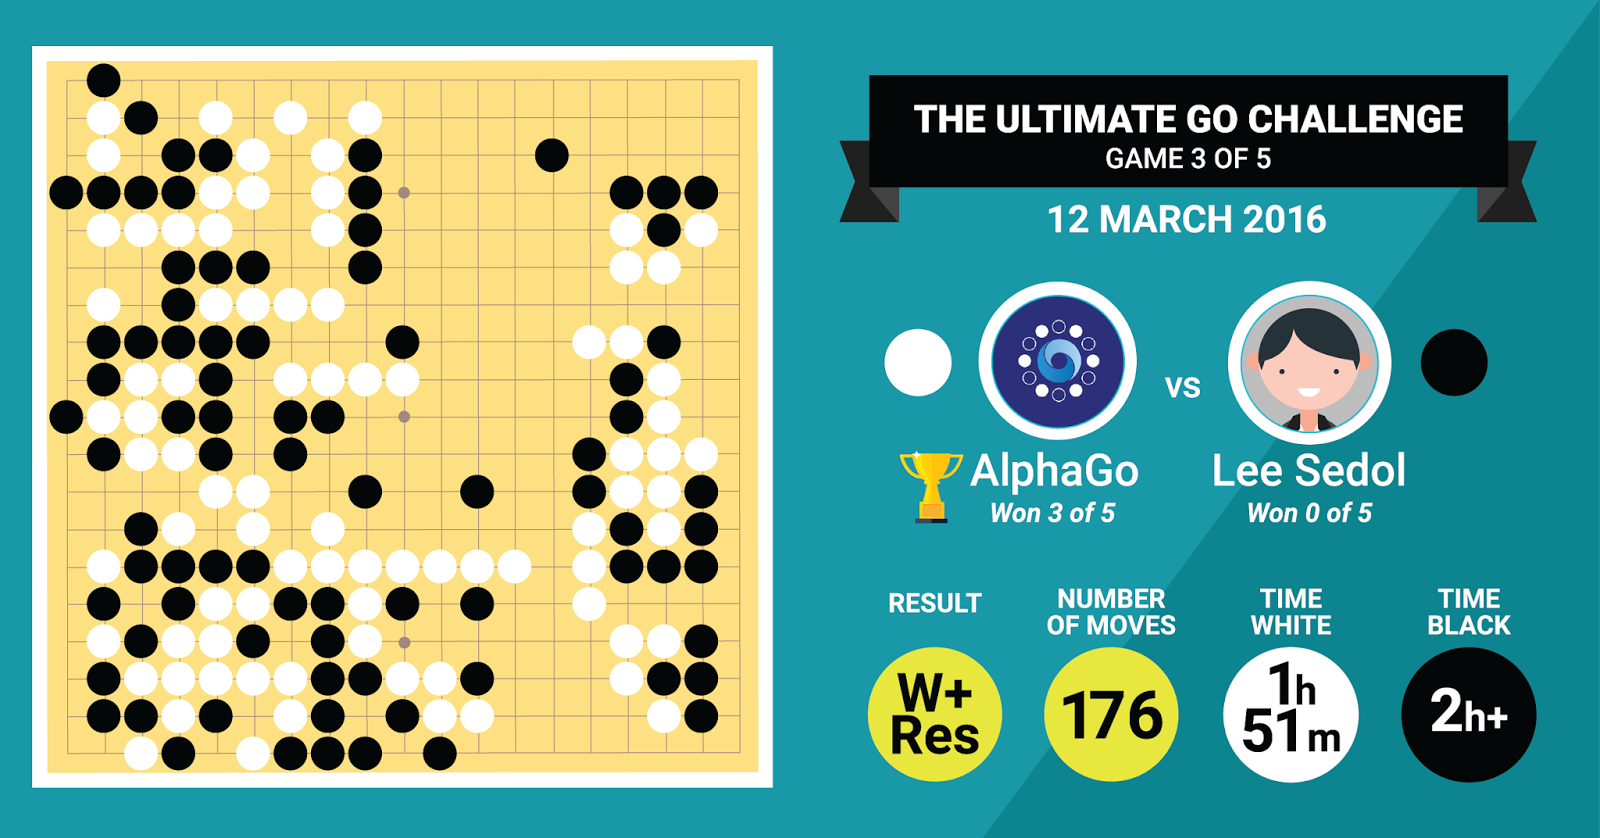
\includegraphics[scale=0.22]{images/alphago.png}
\caption{AlphaGo战胜人类棋手李世石}
\label{fig:alphago}
\end{figure}

自然语言处理与深度学习的初次结合来源于2013年
Mikolov等人\parencite{mikolov2013efficient,le2014distributed,bojanowski2016enriching}提出的Word2Vec模型,
从提出至今,Word2Vec已经成为了深度学习在自然语言处理中的基础部件,
不胜枚举的深度学习模型在表示单词、短语、句子、段落等文本要素时都需要用Word2Vec来做单词级别的向量化。
此后深度学习在自然语言处理领域大显神威,在情感分析\parencite{socher2013recursive}、
问答系统\parencite{li2016deep}、机器翻译\parencite{bahdanau2014neural}等问题上,
以惊人的效果提升,颠覆了使用多年的老方法。
更重要的是,它引起了对主流方法的反思,提供了一个全新的思考视角。

深度学习在推荐系统的应用并不常见,最初的工作来源于2007年Salakhutdinov等人\parencite{salakhutdinov2007restricted}
利用受限莫尔兹曼机(Restricted Boltzmann Machine, RBM)解决Netflix百万美金大奖赛中的电影评分预测任务,
但是之后只有少数几个工作\parencite{phung2009ordinal}继续了该项研究。
当深度学习在图像识别和语音识别领域中取得突破性进展时,开始逐渐有部分工作将深度学习应用于推荐系统中。
Sedhain等人\parencite{sedhain2015autorec}使用自动编码机(AutoEncoder)通过重构评分数据的方式直接进行评分预测,
在多个数据集上取得优异的成绩,但是规避了冷启动的问题,直接使用一个预定义的评分代替那些不能预测的冷启动评分。
Strub等人\parencite{strub2016hybrid}在此基础上进行了改进,使用层叠去燥自动编码机将辅助信息引入进自动编码机学习框架中,
减缓了冷启动造成的负面影响。
Wang等人在\parencite{wang2015collaborative}和\parencite{wang2016collaborative}分别提出
贝叶斯版本的自动编码机和循环神经网络(Recurrent Neural Networks, RNN)来对文本信息进行提取,
融合进概率矩阵分解(Probabilistic Matrix Factorization, PMF)\parencite{salakhutdinov2007probabilistic}的框架中,
在论文推荐场景中取得良好的表现。
2013年Oord等人\parencite{van2013deep},2014年Wang等人\parencite{wang2014improving}
将卷积神经网络引入推荐系统中,从音乐内容的角度出发,解决音乐推荐问题。

\section{本文研究意义}
推荐系统是一个具有很强现实价值的研究领域,优秀的推荐系统不仅可以帮助用户快速获取到感兴趣的物品,
还可以提高物品提供商的转化效率。在当前流行的各类大型网站平台上,
一般都提供了推荐系统的功能方便用户获取自己感兴趣的信息,比如淘宝网站上的商品推荐,或者豆瓣电台中的音乐推荐等。

深度学习是近年来兴起的机器学习范式,通过特定的神经网络结构,直接从原始数据向预测目标进行端到端的转换,
省去了大量的构建特征工程的人力花销,在语音识别、图像识别等诸多研究领域上取得了突破性的进展。

本文正是深度学习应用于推荐系统领域的一次尝试,通过多层感知器模型和长短期兴趣模型解决了电影评分预测任务,
为推荐算法提供了一个新的解题角度。多层感知器模型是一个通用的回归框架,将原始的用户表示和电影表示直接作为输入,
通过多层的神经网络结构一层层地抽象归纳用户和电影的关系,最终得到待预测评分数据。
与此同时,如果真实的推荐环境中还包含各类辅助信息,也可以不进行处理直接加入到多层感知器模型中。

长短期兴趣模型是对传统协同过滤算法的一种扩展。传统的协同过滤算法将同一个用户的交互数据等同视之,这样假设往往是存在问题的。
例如在电商平台上的推荐系统中,采用协同过滤算法时,我们会认为一个用户购买过的商品具有类似的兴趣分布,但实际上随着时间的推移,
用户购买的商品在不同的时间区间往往具有很大的区别。长短期兴趣模型正是用来刻画用户兴趣随时间漂移的现象的一种模型,
在利用评分数据的同时,额外引入了评分时间的信息,让刻画用户兴趣漂移成为了可能,深度学习的框架也保证了可以学习出较好的用户表示和物品表示。
一方面这些较好的用户表示和物品表示可以用在评分预测任务上,另一方面,这些表示还可以帮助发现相似用户和相似电影,
或者异常用户和异常电影,并进行相应的好友推荐或者异常检测等等。

\section{本文主要工作及成果}
本文是深度学习在推荐系统领域应用的一种尝试,提出了多层感知器模型和长短期兴趣模型解决电影评分预测任务,
同时实现了电影推荐原型系统MovieRec用以展示直观的推荐效果。主要包含以下几点成果:

\begin{itemize}
\item
本文利用经典的神经网络结构实现了多层感知器模型,取得了和传统推荐算法相近的实验结果,证明了深度学习应用于推荐系统领域的可行性。
\item
本文针对用户的兴趣分布会随时间流逝发生变化的特点,提出长短期兴趣模型,
在学习过程中融入了时间因素,使得用户模型和物品模型更加具有时效性,从而进一步提升推荐系统的推荐性能。
\item
本文实现了一个电影推荐原型系统MovieRec,将我们提出的多层感知器模型和长短期兴趣模型进行了应用,
可以帮助用户快速发现其可能感兴趣的电影。
\item
本文提出的长短期兴趣模型已经投稿并发表在了第五届自然语言处理与中文计算会议上(NLPCC 2016)。
\end{itemize}

\section{本文篇章结构}
本文一共由六个章节组成。

第一章节是绪论部分,主要介绍了推荐系统和深度学习的研究背景,阐述了本文的研究意义,
然后介绍了我们的主要工作和研究成果,最后描述了本文的篇章结构。

第二章节阐述了推荐系统和深度学习的相关工作,主要包括多种推荐算法的简介,推荐系统的评价方法,
神经网络版本词向量模型,深度学习在推荐系统中的应用实例等相关方法。

第三章节描述了本文提出的基于深度学习的推荐系统算法,主要包含多层感知器模型和长短期兴趣模型。
对于前者,主要介绍了UM模型和U-M模型的算法框架,同时引入了Dropout技术提升算法鲁棒性;
对于后者,主要阐述了如何利用长期兴趣和短期兴趣生成带时序特征的用户表示和电影表示,
并且利用基于特征的矩阵分解框架融合两种表示,最终得到待预测评分的过程。

第四章节展示了本文提出的多层感知器模型和长短期兴趣模型在两类真实世界数据集上的实验效果,
对实验设置、评价方法和实验结果都进行了详细的分析和讨论。

第五章节介绍了基于多层感知器模型和长短期兴趣模型以及其他多种推荐算法的电影推荐系统,
分阶段详细介绍了该原型系统的系统结构,并结合具体用例进行了系统展示。

最后,第六章节对本文的研究工作进行了总结与归纳,并对未来可能的拓展方向进行了展望。



	\chapter{相关工作}
在本章节中,我们主要简单介绍和本文内容相关的研究工作。首先从推荐系统出发,介绍了推荐系统算法的分类情况,
从不同的角度阐述了各类推荐系统的优缺点。然后又讲解了推荐系统中常用的评价算法,包括用户满意度、
预测准确率和一些其他指标。紧接着,我们阐述了词向量表示模型的算法细节,这也是本文提出长短期兴趣模型的灵感来源。
最后,我们简单介绍了部分已经成功将深度学习应用到推荐系统领域的一些工作。

\section{推荐系统的分类}
目前存在的推荐系统可以大致分为三个类别:基于内容的推荐系统(只使用用户画像信息和物品描述信息),
基于协同过滤的推荐系统(只使用评分数据信息)和混合的推荐系统(同时使用两种信息)。

\subsection{基于内容的推荐系统}
基于内容的推荐系统是最早被使用的推荐算法,它根据用户过去喜欢的物品,为用户推荐和它过去喜欢的物品相似的物品。
例如,一个推荐电影的系统可以根据某个用户之前喜欢看喜剧电影而为他推荐新出品的喜剧电影。
该算法的核心假设是``一个用户可能会喜欢和他曾经喜欢过的物品相似的物品'',
这里的相似的物品是通过物品的内容属性来确定的。在不同的推荐场景中,物品的内容属性往往是不同的。
电影推荐中,被推荐的物品是电影,其属性包括导演、演员、风格和发布年份等。
音乐推荐中,被推荐的物品是音乐,其属性包括歌手、曲风、语种和音乐时长等。
商品推荐中,被推荐的物品是商品,其属性包括种类、价格、销量和上市时间等。

基于内容的推荐系统具有良好的解释性,可以告诉用户为什么会给他推荐这些物品,同时不存在物品冷启动问题,
当推荐平台上出现新物品时,也可以做出很好的推荐。但是基于内容的推荐系统只能进行有限的内容分析,
可以提取一些容易提取的物品属性,但对于多媒体数据(图片、、声音、视频等)存在技术上的困难。
而且不能为用户发现新的感兴趣的物品,只能发现和已有兴趣相似的物品,不具有良好的新颖性。

基于内容的推荐系统的过程一般包括以下三个步骤:
\begin{enumerate}
\item \textbf{物品建模:} 通过物品的内容属性,为每个物品抽取一些特征,来表示该物品。
\item \textbf{用户建模:} 利用用户曾经喜欢及不喜欢的物品的特征信息,加权整合出该用户的特征信息,来表示该用户。
\item \textbf{推荐生成:} 通过比较用户模型和候选物品模型的相关程度,为该用户推荐一组相关度最大的物品。
\end{enumerate}
其中物品的内容属性主要分为两类:结构化的属性和非结构化的属性。
所谓结构化的属性就是这个属性的意义比较明确,其取值限定在某个范围内,
而非结构化的属性意义比较模糊,取值也没有限制,难以直接使用。
以电影推荐为例,电影的导演,演员、风格和发布年份都是结构化属性,而电影的剧情介绍等文本信息就属于非结构化属性。
对于结构化信息,我们可以直接将其加到物品特征向量中,而对于非结构化信息,
一个常见的方法是将其转化为向量空间模型(Vector Space Model),
例如我们可以将电影的剧情介绍的文本信息转化为一个长度为词汇表大小的向量,
该向量的每一个维度表示对应词语的权重,TF-IDF是一个常见的权重表示方法,其公式如下:
\begin{equation}
TF\textrm{-}IDF(t_i, d_j) = TF(t_i, d_j) \cdot \log{ \frac{N}{n_i} }
\end{equation}
其中$TF(t_i, d_j)$是第$i$个词语在第$j$篇文档中出现的次数,$N$是所有文档的数量,$n_i$是包含第$i$个词语的文档数量。
通常我们需要进行归一化以便将不同文档的向量统一到一个数量级上,其公式如下:
\begin{equation}
w(i, j) = \frac{ TF\textrm{-}IDF(t_i, d_j) }{ \sqrt{\sum_{k=1}^{T}{TF\textrm{-}IDF(t_k, d_j)^2}} } 
\end{equation}
其中$T$代表所有词语的数量。学术界提出了多种计算用户模型和物品模型相似度的算法,
其中最著名的就是cosine相似度,其公式如下:
\begin{equation}
sim(d_i, d_j) = \frac{ \sum_k{ w(k, i) \cdot w(k, j) } }
{ \sqrt{\sum_{k}{w(k, i)^2}} \cdot \sqrt{\sum_{k}{w(k, j)^2}} } 
\end{equation}
当然,真正的推荐系统中使用的策略往往可以很复杂,比如在用户建模时考虑时间因素,
计算不同时间段内的用户模型,从而发现用户兴趣在历史数据上表现出的偏好变化。
又比如再推荐生成的过程中,使用决策树、支持向量机和神经网络等更高级的模型,
这些方法最核心的环节就是利用用户模型和物品模型之间的相似度进行计算,
因为基于内容的推荐系统不是本文研究的重点,所以在此不加赘述。

\subsection{基于协同过滤的推荐系统}
协同过滤(Collaborative Filtering)算法是推荐系统中应用最为广泛和成功的算法,与传统的基于内容的推荐系统不同,
协同过滤算法分析用户的兴趣,在用户群中找到给定用户的相似用户,综合相似用户对某一信息的评价,
形成系统对该指定用户对此信息的喜好程度预测。与传统的基于内容的推荐系统相比,协同过滤算法
能够处理难以获取内容信息的物品推荐,比如图片、音乐、视频等,还可以保证较高的推荐的新颖性。
但是,当用户对物品的评价数据较为稀疏时,协同过滤算法推荐效果较差。随着用户和物品数量的增多,
协同过滤算法的性能会越来越低,同时冷启动问题也是协同过滤算法难以解决的,
当新用户或者新物品出现在推荐平台上时,协同过滤算法无法做出有效的推荐。

基于协同过滤的推荐系统可以分为三个子类:基于用户的协同过滤,基于物品的协同过滤和基于模型的协同过滤。
\subsubsection{基于用户的协同过滤}
研究生生活中,我们往往会向实验室的老师咨询该阅读哪些论文,老师也会给出一些推荐,
往往这些推荐都是我们想要的,其主要原因是我们和老师有着共同的研究领域和兴趣。
在一个在线的推荐系统中,当一个用户需要个性化推荐时,可以先找到和他兴趣相似的其他用户,
然后将那些用户偏爱的而且当前用户没有听说过的物品进行推荐,这种方法就是基于用户的协同过滤算法。

基于用户的协同过滤算法的核心是计算用户之间的兴趣相似度,而兴趣相似度一般是使用行为相似度来进行模拟。
给定用户$u$和用户$v$,假设$N(u)$代表用户$u$曾经偏爱过的物品集合,而$N(v)$代表用户$v$曾经偏爱过的物品集合,
那么我们可以通过如下的Jaccard公式简单计算用户$u$和用户$v$之前的行为相似度:
\begin{equation}
sim(u, v) = \frac{ |N(u) \cap N(v)| } { |N(u) \cup N(v)| }
\end{equation}
或者通过余弦相似度来计算:
\begin{equation}
sim(u, v) = \frac{ |N(u) \cap N(v)| } { \sqrt{ |N(u)| |N(v)| } }
\end{equation}
得到用户之间的兴趣相似度之后,基于用户的协同过滤算法会给用户推荐和他兴趣最相似的$K$个用户喜欢的物品,
如下的公式度量了用户$u$对物品$i$的感兴趣的程度:
\begin{equation}
p(u, i) = \sum_{v \in S(u, K) \cap N(i) }{ sim(u, v) }
\end{equation}
其中,$S(u, K)$代表和用户$u$兴趣最相似的$K$个用户,$N(i)$是对物品$i$偏爱的用户集合,
$sim(u, v)$表示用户$u$和用户$v$的兴趣相似度。

\subsubsection{基于物品的协同过滤}
基于物品的协同过滤算法在目前工业界中应用广泛,给用户推荐和那些他们之前偏爱过的物品相似的物品,
和基于内容的推荐系统不同的是,该算法不利用物品的内容属性计算物品之间的相似度,
而是通过分析用户的行为数据来计算物品之间的相似度,它认为物品$A$和物品$B$具有很大的相似度取决于喜欢物品$A$
的用户大都也喜欢物品$B$。

和基于用户的协同过滤算法类似,基于物品的协同过滤算法的核心是计算物品之间的兴趣相似度,
也是使用行为相似度进行模拟。
给定物品$i$和物品$j$,假设$N(i)$代表喜欢过物品$i$的用户集合,而$N(j)$代表喜欢过物品$j$的用户集合,
那么我们可以通过如下的Jaccard公式简单计算物品$i$和物品$j$之前的行为相似度:
\begin{equation}
sim(i, j) = \frac{ |N(i) \cap N(j)| } { |N(i) \cup N(j)| }
\end{equation}
或者通过余弦相似度来计算:
\begin{equation}
sim(i, j) = \frac{ |N(i) \cap N(j)| } { \sqrt{ |N(i)| |N(j)| } }
\end{equation}
得到物品之间的兴趣相似度之后,基于物品的协同过滤算法会给用户推荐和喜欢过的物品兴趣最相似的$K$个物品,
如下的公式度量了用户$u$对物品$i$的感兴趣的程度:
\begin{equation}
p(u, i) = \sum_{j \in S(i, K) \cap N(u) }{ sim(i, j) }
\end{equation}
其中,$S(i, K)$代表和物品$i$兴趣最相似的$K$个物品,$N(u)$是用户$u$喜欢过的物品集合,
$sim(i, j)$表示物品$i$和物品$j$的兴趣相似度。

\subsubsection{基于模型的协同过滤}
基于模型的协同过滤算法中最经典的当属矩阵分解算法,在成功解决Netflix百万美金大奖赛后的数十年内,
矩阵分解算法在学术界和工业界都备受关注和研究。在电影评分预测任务中,
已观察到的评分数据可以构成一个$N \times M$的大型稀疏矩阵,$N$代表用户数量,$M$代表电影数量,
该矩阵可以分解成$Q$和$P$两个低秩子矩阵相乘,其中子矩阵$Q$的大小为$N \times K$,代表用户因子矩阵,
子矩阵$P$的大小为$K \times M$,代表电影因子矩阵,$K$代表隐因子的数量。

\begin{figure}[htbp]
\centering
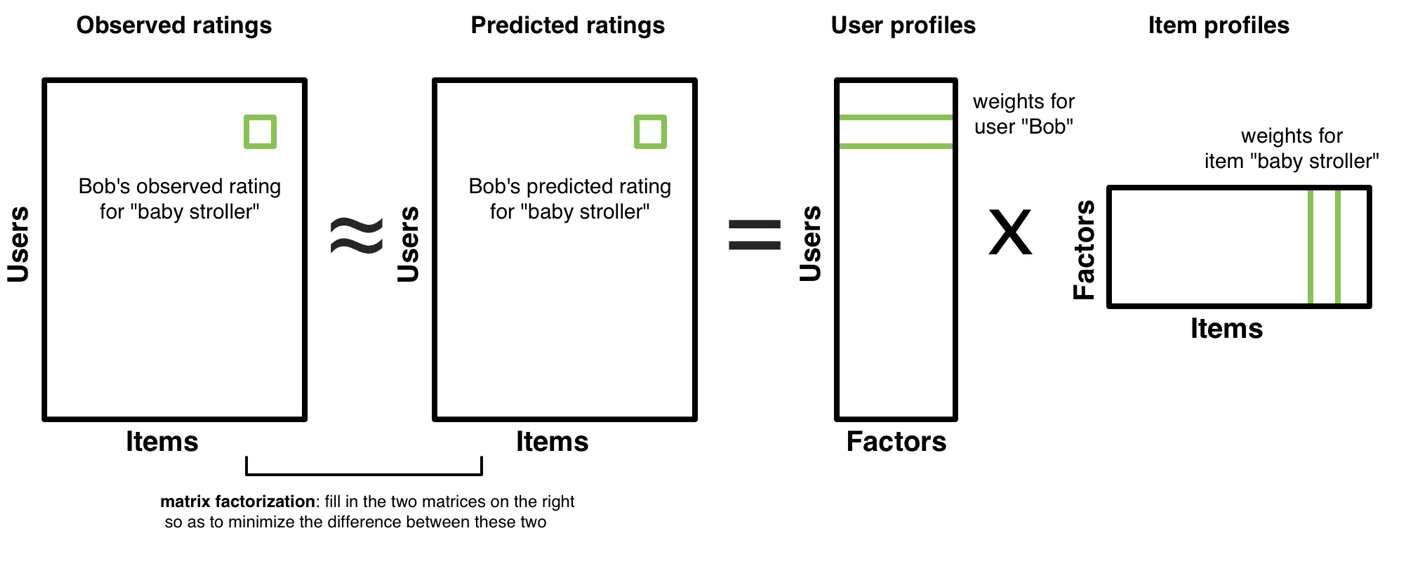
\includegraphics[scale=0.6]{images/mf.png}
\caption{基于矩阵分解的协同过滤算法}
\label{fig:mf}
\end{figure}

如图\ref{fig:mf}所示,第一个矩阵代表原始的大型稀疏矩阵,其中包含已观察到的评分数据和待预测的评分数据,
第三个和第四个矩阵代表用户因子矩阵和电影因子矩阵,在矩阵分解训练的过程中,
我们使两个子矩阵相乘的结果尽可能地去接近原始矩阵中已观察到的评分数据,而不去关心待预测的评分数据,
从而通过原始矩阵生成出这两个子矩阵。第二个矩阵代表生成完两个子矩阵后,两个子矩阵再相乘还原出来的预测矩阵,
该预测矩阵和原始矩阵大小相同,对应的评分位置上,已观察的评分数据和原始矩阵十分接近,
待预测的评分数据也计算出来相应的预测结果,评分预测的任务也自然得到了解决。

具体的训练过程中,我们首先随机初始化用户子矩阵和电影子矩阵,然后定义如下的优化目标:
\begin{equation}
\min_{q*, p*} \sum_{(u, i) \in \mathcal{K} }{ (r_{ui} - q_i^T \cdot p_j)^2 + \lambda (|q_i|^2 + |p_j|^2) }
\end{equation}
其中$\mathcal{K}$代表已观察到的评分数据集合,$r_{ui}$代表观察到的用户$u$给电影$j$的评分数据,
$q_i^T \cdot p_j$代表两个子矩阵相乘后对应的预测评分数据,$\lambda (|q_i|^2 + |p_j|^2)$是保证算法鲁棒性的正则化项。
从该公式我们可以看出,优化目标是使得两个子矩阵的乘积在已观察评分数据上和原始矩阵的差值尽可能的小。
一般会采用随机梯度下降进行算法训练,具体的更新公式为:
\begin{equation}
e_{ui} = r_{ui} - q_i^T \cdot p_u
\end{equation}
\begin{equation}
q_i \leftarrow q_i + \gamma \cdot (e_{ui} \cdot p_u - \lambda \cdot q_i)
\end{equation}
\begin{equation}
p_u \leftarrow p_u + \gamma \cdot (e_{ui} \cdot q_i - \lambda \cdot p_u)
\end{equation}

\subsection{混合的推荐系统}
由于不同的推荐算法各有利弊,所以在实际的应用场景中,单纯一种推荐策略往往并不能满足推荐需求。
工业界的具体实现中,人们常常将多个方法进行混合,从而达到更好的推荐效果。
关于如何混合不同的推荐策略,这里简单地描述几种比较流行的混合方法。
\begin{itemize}
\item \textbf{加权的混合:}
参考集成学习(Ensemble Learning)的思想,使用若干不同的推荐算法获得多个推荐结果,
然后使用线性结合的方式将这些推荐结果按照一定权重组合起来,最后按照新的权重进行重排序,
产生新的推荐列表。这里的具体权重的数值需要在训练数据集上反复试验,从而达到最好的混合推荐效果。
\item \textbf{分层的混合:}
加权的混合策略可以看成是对多个推荐算法的并联处理,同样我们也可以选择串联处理,
将一个推荐方法的输出作为另外一个推荐方法的输入,以此类推,构成一个串联结构,
从而综合各个推荐策略的优缺点,得到更加准确的推荐结果。
\item \textbf{切换的混合:}
除了将多个推荐模型混合在一起,我们也可以选择在不同的生产环境下选择最适应当前情况的推荐方法。
例如,在商品推荐的场景下,如果发现用户数量超过物品数量,我们可以选择使用基于物品的协同过滤算法,
而当物品数量超过用户数量时,我们切换至基于用户的协同过滤算法。
\item \textbf{分区的混合:}
另外,我们也可以在推荐结果展示界面做文章。采用多种推荐机制,将不同的结果分在不同的区域展示给用户。
例如,亚马逊、淘宝和京东等很多电子商务网站都是采用这样的方式,
用户可以得到很全面的推荐,也会更加容易找到他们想购买的商品。
\end{itemize}

\section{推荐系统的评价}
一个完整的推荐系统一般包含两个参与者:用户和物品。以电影推荐为例,
首先推荐系统需要满足用户的需求,为用户推荐其可能喜爱的电影,
其次,推荐系统也需要满足物品的需求,保证各个电影都有被推荐的机会。
一个良好的推荐系统需要同时考虑两者的利益,构成双方共赢的场面。

在推荐系统中,主要存在三种评价推荐效果的实验方法:离线实验、在线实验和用户调查。

离线实验首先通过日志系统获取用户的行为数据,生成一个标准的数据集,
然后按照一定规则将其切分为训练集和测试集,实验者在训练集上训练推荐模型,
并在测试集上进行预测,最后通过离线评价算法得出推荐模型的预测效果。
离线实验不需要一个实际的系统和真实的用户进行验证,可以进行直接快速的计算,
从而方便进行大量的算法验证,是研究人员的首选方案。
但是离线实验无法得出很多商业模式上关心的点击率和转换率等指标。

在线实验又可以称为AB测试,它通过一定规则将在线用户随机分为两组,
一组采用原始的推荐算法,另外一组使用待验证的推荐算法,
通过统计两组用户的点击率和转化率可以对比待验证算法和原始推荐算法的优劣。
在线测试可以公平地获取不同算法实际在线时的性能指标,
但是其成本开销较大,且必须进行长期的实验才能得到可靠的效果,
不太适用于学术界的研究钻研。

用户调研是随机招募一些真实用户,让他们在待测试的推荐系统上完成一些任务,
实验者观察并记录用户行为,最后让用户回答一些问题,
通过用户行为和用户答案我们可以获知待测试推荐系统的性能。
用户调研需要保证分布真实,比如男女各半,还需要进行双盲实验。
用户调研可以直观得出用户使用过程中的感受,
缺点是很难进行大规模的验证,统计意义不足,容易出现较大的效果偏差。

由于推荐系统应用场景的多样性,历史上研究人员提出了多种评价推荐系统性能的指标,
有些指标可以定量计算,有些只能定性描述。我们下面简单介绍其中有名的几类。

\subsection{用户满意度}
用户满意度是用户对推荐系统效果最直观的评价,其无法通过里县实验计算,
只能通过在线实验或者用户调研获得。
在线实验中,用户满意度一般和用户行为挂钩,
我们既可以在推荐结果列表里添加满意和不满意两种按钮供用户进行直接反馈,
也可以通过点击率,停留时间和转化率等指标进行衡量。
用户调研中,用户满意度一般和用户答案挂钩,
通过设计问卷调查题目,我们可以了解用户对当前推荐系统各个方面的满意程度。

\subsection{预测准确度}
预测准确度是离线实验中最重要的评价指标,其度量推荐系统预测用户未来行为的能力,
主要分为两种:评分预测和TopN预测。

\begin{itemize}
\item \textbf{评分预测}
推荐系统的很多应用场景中,都提供了用户给物品进行评分的功能,
通过评分数据可以反应用户对物品的偏爱程度。
通过用户的历史评分数据,实验者建立推荐模型,预测用户将来的评分数据,
系统系统可以选择其中评分较高的物品进行推荐。
评分预测的预测准确度一般通过均方根误差(Root Mean Square Error, RMSE)
和平均绝对误差(Mean Absolute Error, MAE)计算。
对于测试集T中的每一个用户$u$和物品$i$,假设$r_{ui}$代表用户$u$对于
物品$i$的真实评分,$\hat{r}_{ui}$代表推荐算法的预测评分,
则均方根误差的计算公式为:
\begin{equation}
RMSE = \sqrt{\frac{\sum_{u,i \in T}{(r_{ui} - \hat{r}_{ui})^2}}{|T|}}
\end{equation}
平均绝对误差的计算公式为:
\begin{equation}
MAE = \frac{\sum_{u,i \in T}{|r_{ui} - \hat{r}_{ui}|}}{|T|}
\end{equation}
对比均方根误差和平均绝对误差,
Netflix认为均方根误差加大了对预测不准的评分的惩罚(平方项的惩罚),
因此均方根误差相对平均绝对误差更加苛刻。

\item \textbf{TopN预测}
推荐系统的展示结果一般是一个包含若干物品的个性化推荐列表,我们一般称之为TopN推荐,
其预测准确率一般通过对比个性化推荐物品列表和用户真实喜爱物品列表,
计算准确率(Precision)和召回率(Recall)来实现。
对于测试集T中的每一个用户$u$,假设$R(u)$代表用户$u$真实喜爱的物品列表,
而$\hat{R}(u)$代表推荐给用户$u$的个性化推荐列表,
则准确率的计算公式为:
\begin{equation}
Precision = \frac{ \sum_{u \in T}{|R(u) \cap \hat{R}(u)|} }{ \sum_{u \in T}{|\hat{R}(u)|} }
\end{equation}
召回率的计算公式为:
\begin{equation}
Recall = \frac{ \sum_{u \in T}{|R(u) \cap \hat{R}(u)|} }{ \sum_{u \in T}{|R(u)|} }
\end{equation}
\end{itemize}
准确率体现了在我们推荐的物品列表里面,用户喜爱的占比多少。
而召回率体现了在用户喜爱的物品列表里面,我们推荐的占比多少。
两者都是数值越大,推荐效果越好。
同时,我们也会使用$F1$值来结合准确率和召回率,其计算公式为:
\begin{equation}
F1 = \frac{Precision \cdot Recall}{ \alpha \cdot Precision + (1 - \alpha) \cdot Recall }
\end{equation}
其中,$\alpha$的数值位于0到1之间,用于控制准确率和召回率两者相对的影响因子。

\subsection{其他指标}
同时推荐系统中还包含其他一些评价指标,我们在此简单介绍如下:
\begin{itemize}
\item \textbf{覆盖率}描述了一个推荐系统对长尾物品(Long Tail)的挖掘能力,
可以简单定义为所有推荐出来的物品占总物品集合的比例。具有较高覆盖率的推荐系统不仅可以推荐热门物品,
还可以推荐少数人喜爱的小众物品。
\item \textbf{多样性}描述了推荐列表中物品两两之间的不相似性,
具有较高多样性的推荐系统尽可能满足用户多种兴趣需求。
\item \textbf{新颖性}代表推荐系统为用户推荐了他们以前没有听说过的物品,
在一个网站实现新颖性的最简单的方式就是过滤掉用户之前有过行为的物品。
\item \textbf{惊喜度}表示推荐系统给用户推荐了和其历史上喜欢的物品不相似的物品,
但是却可以令用户感到满意,是一种定性的度量方式。
\item \textbf{信任度}描述了用户对推荐系统给出的推荐结果的信任程度,
具有解释性的推荐结果一般具有较高的信任度。
\item \textbf{实时性}保证推荐系统可以实时地更新推荐列表来满足用户新的行为的变化,
也需要推荐系统能够将新加入推荐平台的新物品可以推荐给用户。
\item \textbf{健壮性}代表推荐系统的抗攻击能力,常见的攻击手段是注入攻击,
利用大量的虚假账号来为自己的物品评非常高的分数,从而欺骗推荐系统。
\end{itemize}

\section{深度学习在自然语言处理中的成功应用}
\subsection{词向量表示}
早期的词向量表示是独热表示法(One-Hot Representation),在高维向量中只有一个维度描述了词语的信息,
没有词序信息,也无法准确地捕捉语义信息,存在严重的``语义鸿沟''现象。例如``卡拉OK''和``麦克风''
在语义上指代同一件物品,但是在独热表示中却无法观察得到。
Hinton等人\parencite{hinton1986learning}在1986年提出分布表示法(Distributed Representation),
其基本思想是 通过训练将每个词映射成$K$维实数向量,
通过向量之间的距离(余弦相似度或欧氏距离等)来判断它们之间的语义相似度。
这样以来,``卡拉OK''和``麦克风''就可以映射到两个距离很近的低维实数向量中,从而体现两者语义相近的关系。

Word2Vec是谷歌公司在2013年开源的一款将词映射为实数向量的高效工具,由Mikolov等人\parencite{mikolov2013efficient}提出。
其利用深度学习的思想,可以通过训练把对文本内容的处理简化为低维实数向量空间中的向量运算,
而向量空间上的相似度可以用来表示文本语义上的相似度。同时,输出的词向量是连续的向量,可以支持使用连续模型做文本处理。
Word2vec输出的词向量可以被用来做很多自然语言处理相关的工作,比如文本聚类、词性分析、机器翻译等等。
训练出的向量有一定的特性,即相近意义的词在向量空间上其距离也是相近,
有一个经典例子就是$V(`king') – V(`man') + V(`woman') \approx V(`queen')$。

Word2Vec是一个用于处理文本的双层神经网络,它的输入是大量的文本语料,输出则是每个词语对应的一个向量表示,
主要包括两个基本模型:CBOW模型和Skip-gram模型。其中CBOW模型使用上下文预测目标词,
而Skip-gram模型则是用一个词来预测一段上下文。

\begin{figure}[htbp]
\centering
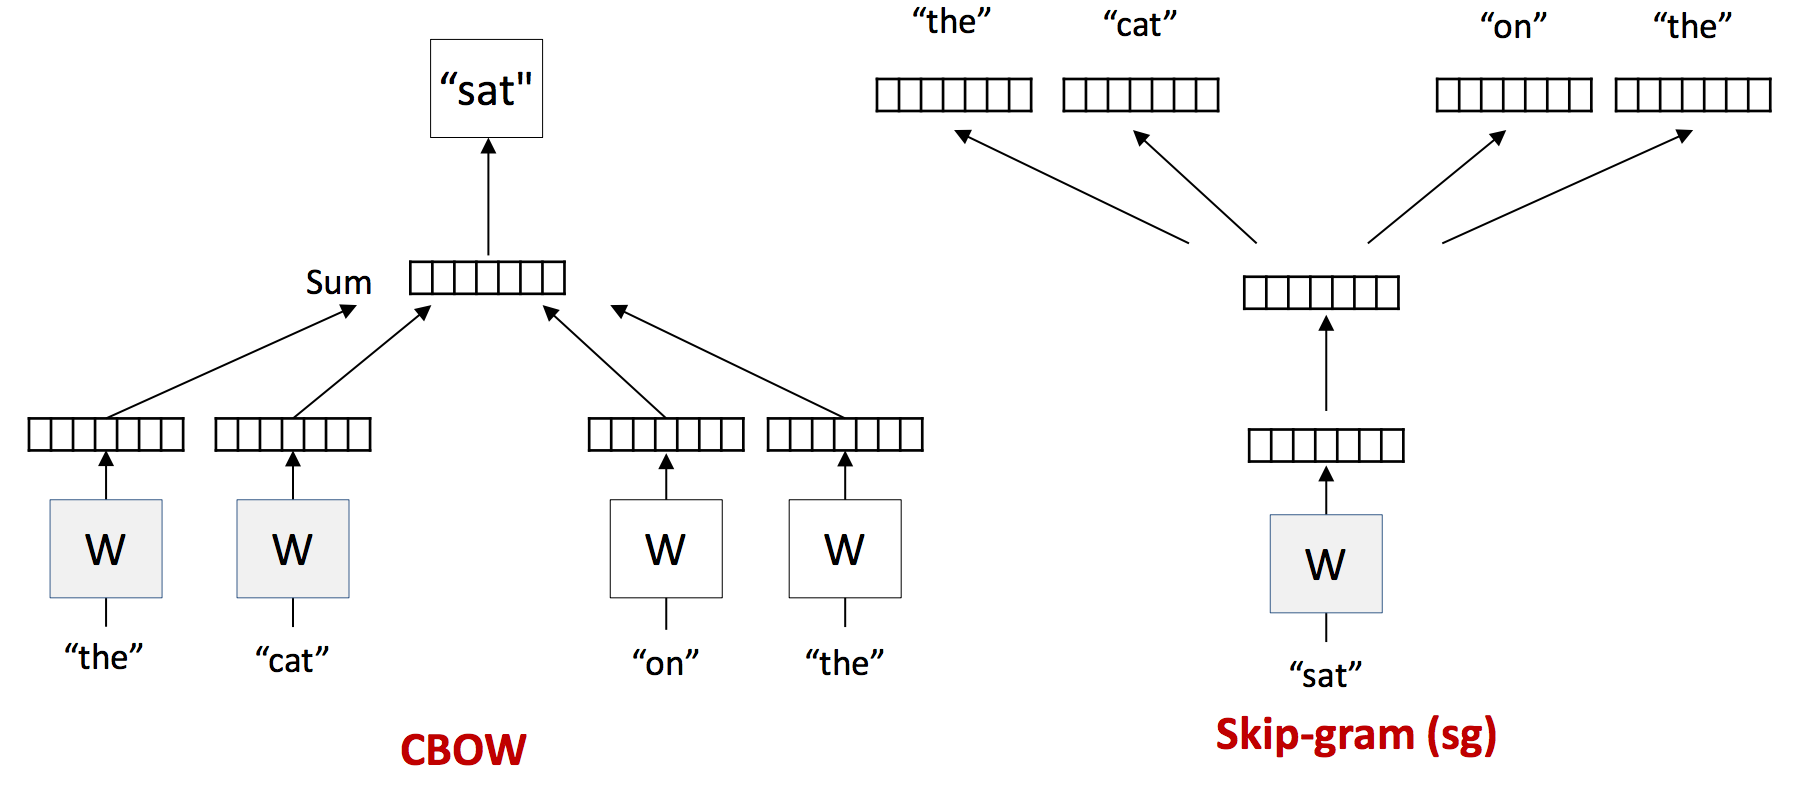
\includegraphics[scale=0.4]{images/w2v.png}
\caption{Word2Vec中的CBOW模型和Skip-gram模型示意图}
\label{fig:word2vec}
\end{figure}

图\ref{fig:word2vec}展示了CBOW模型和Skip-gram模型的示意图,左半部分代表CBOW模型,
``the'', ``cat'', ``on''和``the''是一个语义窗口内的上下文,``sat''是目标词,
每个词语会被赋予一个长度为$K$的随机初始化的向量进行表示,上下文通过聚合的方式形成一个整体,
然后对目标词进行预测,预测过程中的误差会被反向传播回来对上下文的词向量进行更新,直到最后收敛,
从而完成训练过程。具体来说,CBOW模型的目标函数是:
\begin{equation}
Loss = \sum_{t=1}^T {\log P(w_t| w_{t-c} : w_{t+c}) }
\end{equation}
这里的$T$代表训练语料中的所有词语的数量,$c$表示上下文的窗口大小,$w_{t-c} : w_{t+c}$除了$w_t$本身的上下文序列。
似然概率$P(w_t| w_{t-c} : w_{t+c})$使用softmax定义,上下文序列的聚合可以使用向量和或者向量均值来实现。

右半部分代表Skip-gram模型,和CBOW模型不同的是,其使用当前词语来预测上下文,
``sat''是当前词,``the'', ``cat'', ``on''和``the''是一个语义窗口内的上下文,
同样地,每个词语会被赋予一个长度为$K$的随机初始化的向量进行表示,当前词语作为输入对上下文中的所有词语进行预测,
预测过程中的误差会被反向传播回来对当前词语的词向量进行更新,直到最后收敛,从而完成训练过程。
具体来说,Skip-gram模型的目标函数是:
\begin{equation}
Loss = \sum_{t=1}^T {\log P(w_{t-c} : w_{t+c} | w_t) }
\end{equation}
这里的$T$代表训练语料中的所有词语的数量,$c$表示上下文的窗口大小,$w_{t-c} : w_{t+c}$除了$w_t$本身的上下文序列。
似然概率$P(w_{t-c} : w_{t+c} | w_t)$也是使用softmax定义.

\subsection{句向量表示}
2014年Le等人\parencite{le2014distributed}在Word2Vec的基础上提出了Doc2Vec模型,其原理与Word2Vec非常的相似。
Doc2Vec也包括两个基本模型,分别是DM模型和DBOW模型,如图\ref{fig:doc2vec}所示。

\begin{figure}[htbp]
\centering
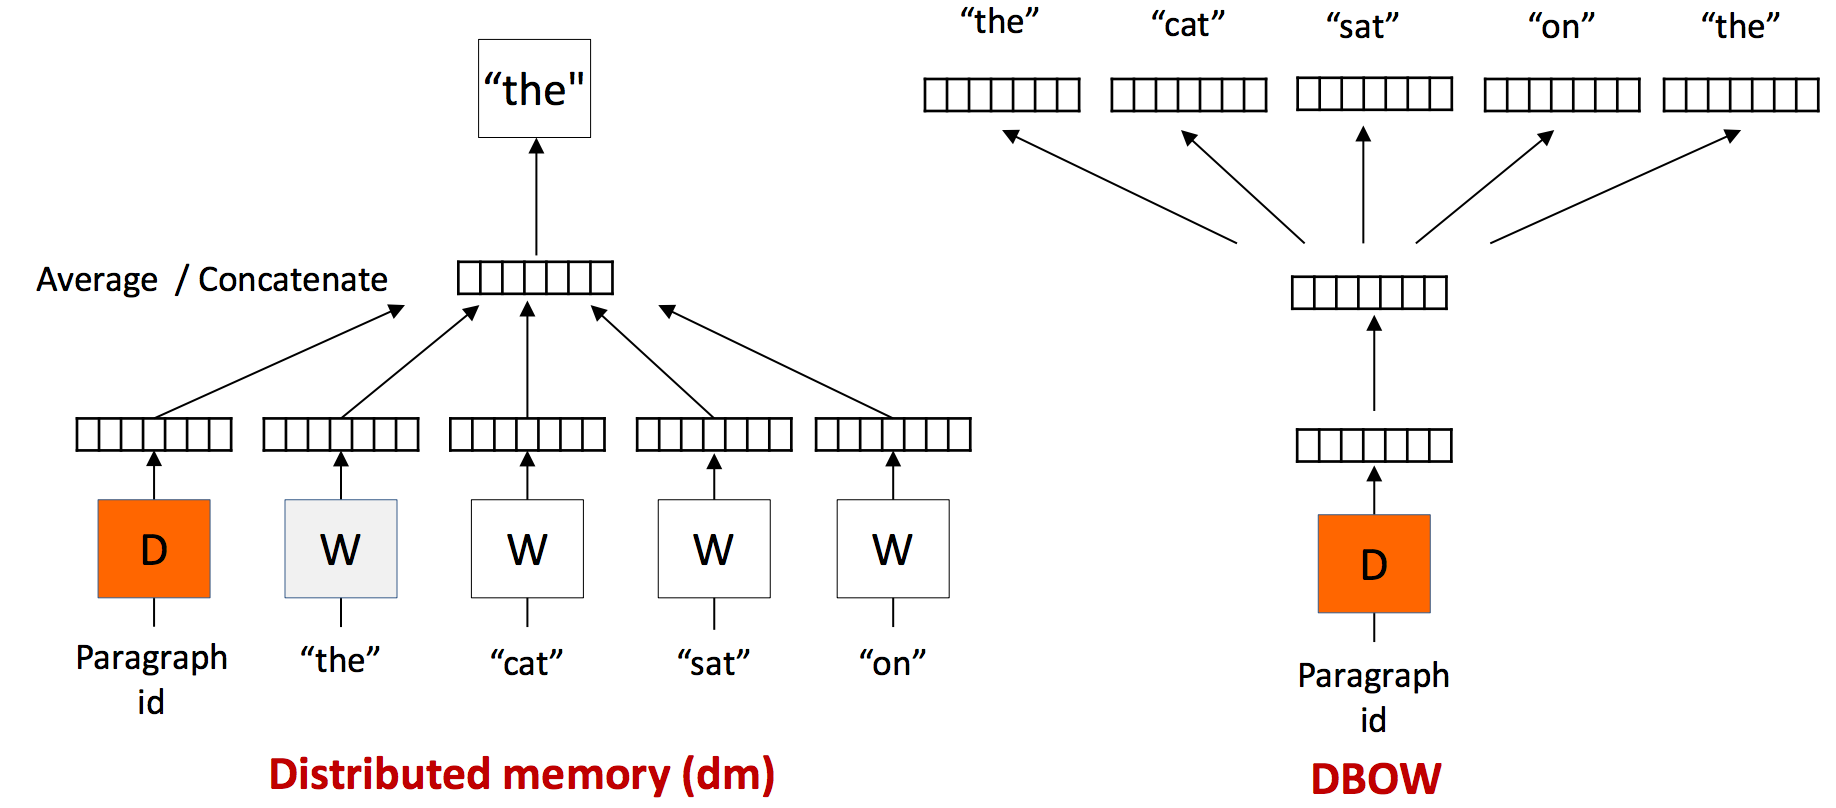
\includegraphics[scale=0.4]{images/d2v.png}
\caption{Doc2vec中的DM模型和DBOW模型示意图}
\label{fig:doc2vec}
\end{figure}

可以看出DM模型和CBOW模型方法类似,DBOW模型和Skip-gram模型方法类似。
不同于Word2Vec的是,Doc2Vec在整个模型中引入了句向量表示,即每一个句子也拥有一个向量表示。
图中的左半部分是DM模型,其在使用上下文预测目标词的同时额外加上了一个全局的句子向量作为输入信息,
而右半部分是DBOW模型,使用句子向量去预测上下文。
因为Doc2Vec算法和Word2Vec算法十分类似,这里不再赘述。

\section{深度学习在推荐系统中的成功应用}
自从深度学习在语音识别和图像识别领域取得突破性进展后,不少研究领域开始尝试在自己领域中引入深度学习,
推荐系统也不例外,在本章节中我们会从自动编码机和循环神经网络两个模型出发介绍深度学习在推荐系统中的成功应用。

\subsection{自动编码机}
自动编码机(Autoencoder)是一种特殊的神经网络结构,最简单的自动编码机由三层网络组成,
分别是输入层,隐藏层和输出层。其中输入层神经元数量与输出层神经元数量相等,隐藏层神经元数量少于输入层和输出层。
自动编码机的训练目标是是的输出信息和输入信息尽可能相似,因为隐藏层神经元数量较少,
所以在数据从输入层到隐藏层的过程可以看成是一种压缩行为,也可以理解为对输入数据的一种编码过程;
而从隐藏层到输出层可以看成数据的解压缩行为,也可以理解为对隐藏层数据的一种解码过程。
因为隐藏层瓶颈的存在,迫使自动编码机学习了对原始输入数据进行压缩提取的一个过程。

Sedhain等人\parencite{sedhain2015autorec}最早提出使用自动编码机通过重构评分数据的方式直接进行评分预测,
Strub等人\parencite{strub2016hybrid}在此基础上进行了改进,
提出了如图\ref{fig:ae}所示的CFN(Collaborative Filtering Neural network)模型,
将噪音去除机制引入训练过程中,极大增强了整个模型的鲁棒性,

\begin{figure}[htbp]
\centering
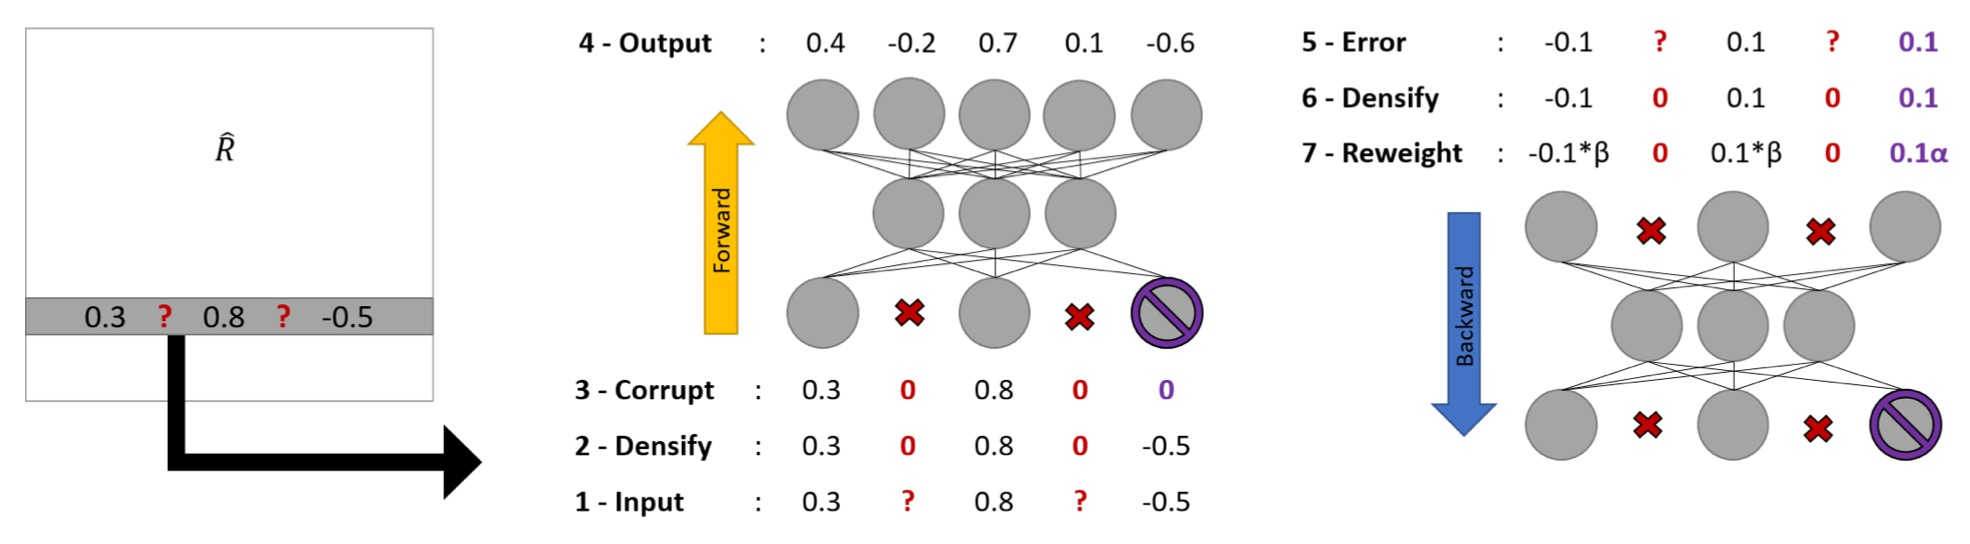
\includegraphics[scale=0.22]{images/ae.jpeg}
\caption{自动编码机}
\label{fig:ae}
\end{figure}

图中的左边部分代表原始的大型稀疏矩阵,CFN模型会对其中的数据进行分行处理,
即将每一个用户的所有评分作为一个样本输入进自动编码机中。
如果从物品的角度出发,CFN模型就会进行分列处理,将每一个物品的所有评分作为一个样本输入进自动编码机中。
图中的中间部分表示CFN模型的正向传播过程。评分数据主要分为已观察到的评分和待预测的评分两类。
对于已观察到的评分,CFN模型会以一定的概率将其变成噪声数据,如图中的紫色节点表示的``-0.5''分被变成了噪声数据``0''分;
对于待预测的评分数据,CFN模型会将其进行标记,从而在训练优化过程中将其忽略,如图中的红色叉型节点。
图中的右边部分代表CFN模型的误差反向传播过程,对于待预测的评分CFN模型将其从误差函数中去除,
对于已观察到的数据,分为是否是噪声数据进行不同权重的误差累计,
图中紫色节点的误差被乘以系数$\alpha$作为修改后的误差,而灰色节点的误差被乘以系数$\beta$作为修改后的误差,
红色节点的误差则被忽略。

通过这样的过程,CFN模型利用自动编码机从输入数据中重构出那些被变成噪声数据的评分,
从而学习出不同用户评分数据之间的关系。完成训练后,我们可以将输出层中的待预测评分数据作为预测结果。
另外图中的自动编码是只包含一个隐藏层,CFN模型还可以增加网络的深度,学习出更加深层的数据关系。
最后,CFN还提出了在输入层加入辅助信息的方式来减缓推荐系统中的冷启动问题,
实验结果证明加入辅助信息对评分较少的用户和物品都有较大的预测准确度提升。

CFN模型和本文方法都是使用定制的神经网络结构对推荐问题进行建模,不同的是他们采用了自动编码机,而我们使用了多层感知器。
相比较而言,相同实验设定下,自动编码机模型的参数规模大约是多层感知器的两倍,主要因为自动编码机包含编码层和解码层,
而多层感知器只有编码层;但由于噪声机制的引入,CFN模型除了具备数据还原能力和数据去噪能力,
在预测准确度和鲁棒性上都高于多层感知器。

\subsection{循环神经网络}
循环神经网络是一种特殊的神经网络结构,在处理序列数据上有着其得天独厚的优势,通过隐藏层节点保存历史序列信息,
并在每次迭代中融入新的信息,从而完成序列标注,分类预测等任务。
循环神经网络并不能很好地处理较长的序列,一个改进版本的循环神经网络是LSTM(Long Short Term Memory),
通过加入输入门、遗忘门和输出门,LSTM可以刻画较长序列中的远距离依赖问题。

\begin{figure}[htbp]
\centering
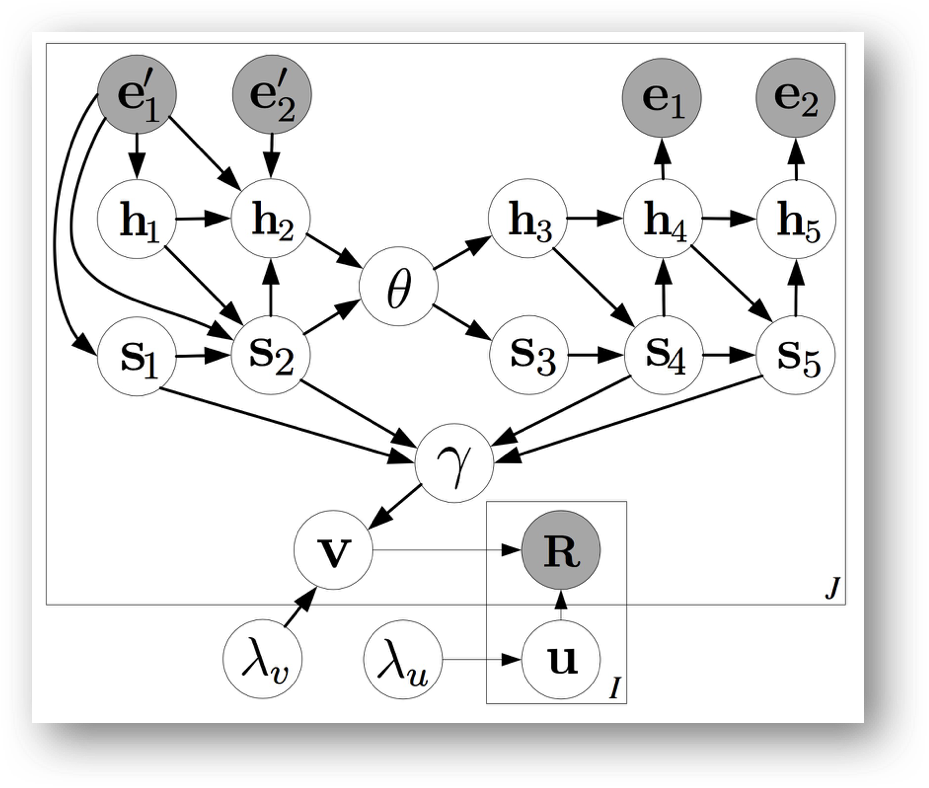
\includegraphics[scale=0.6]{images/pmf_rnn.png}
\caption{循环神经网络}
\label{fig:pmf_rnn}
\end{figure}

循环神经网络在很多自然语言处理任务中取得了巨大成功以及广泛应用,例如文本分类,机器翻译,对话模型等等。
Wang等人\parencite{wang2016collaborative}提出贝叶斯版本的循环神经网络来对论文摘要文本信息进行提取,
然后将其加入到概率矩阵分解中,在论文推荐任务中取得优异的性能表现,整个算法框架如图\ref{fig:pmf_rnn}所示。

图中上半部分表示循环神经网络对论文摘要信息进行提取,其中``e''节点代表文本信息中的一个个单词,
``h''节点和``s''节点分别代表LSTM中的隐藏节点和状态节点,在该网络结构中,
循环神经网络首先接受一段文本输入,逐步将每个单词信息编码进隐藏节点和状态节点中,
然后通过中间的一个瓶颈节点``$\theta$''进行压缩和解压缩,再逐步将每个单词信息解码输出出来。
这是一个典型的``seq-to-seq''框架,通过重构本身数据的方式将文本信息融入到神经网络的节点中。
紧接着,使用``$\gamma$''节点聚合了所有的隐藏节点和状态节点信息,这里可以看成是加权求和,
然后综合``$\lambda_v$''节点生成了``$v$''节点,即物品节点。
最后物品节点``$v$''和用户节点``$u$''进行组合,得到评分节点``$R$''。
整个框架中,所有的灰色节点是已知数据,即评分数据和文本信息,所有的白色节点是待学习的数据,
包括用户节点和物品节点等。因为是贝叶斯网络结构,所以训练过程通过最大后验概率实现。

相对于传统的词袋模型,Wang等人提出的方法中的循环神经网络可以更好地刻画文本数据之间的序列关系,
从而保证学习出来的文本信息更加地准确和丰富,多项实验结果也证明了该算法的有效性。
和Wang等人工作不同的是,我们并没有利用这些文本信息数据,而是利用用户的评分时间信息对物品相似度进行建模。
Wang等人的工作可以看成是基于内容的方法的一种实现,本文的工作则是基于协同过滤的方法的一种实现。
在文本信息较为丰富的场景下,如论文推荐、图书推荐等,Wang等人的工作更加具备优势,
而在文本信息较为稀缺的场景下,如商品推荐、音乐推荐等,我们的工作则更加适用。



	\chapter{基于深度学习的个性化推荐}

协同过滤算法的基本假设是,被相同用户偏爱的物品具有相似的兴趣分布,
或者喜欢相同物品的用户拥有相似的兴趣分布。然而在现实的环境中,
由于用户的兴趣会随着时间发生变化(兴趣漂移),这样的假设并不总是成立。
但是从另外一个角度而言,对于一个给定的用户,在一个给定的时间段内,
该用户的兴趣分布往往是稳定的,不会发生剧烈的变化。

\begin{figure}[htbp]
\centering
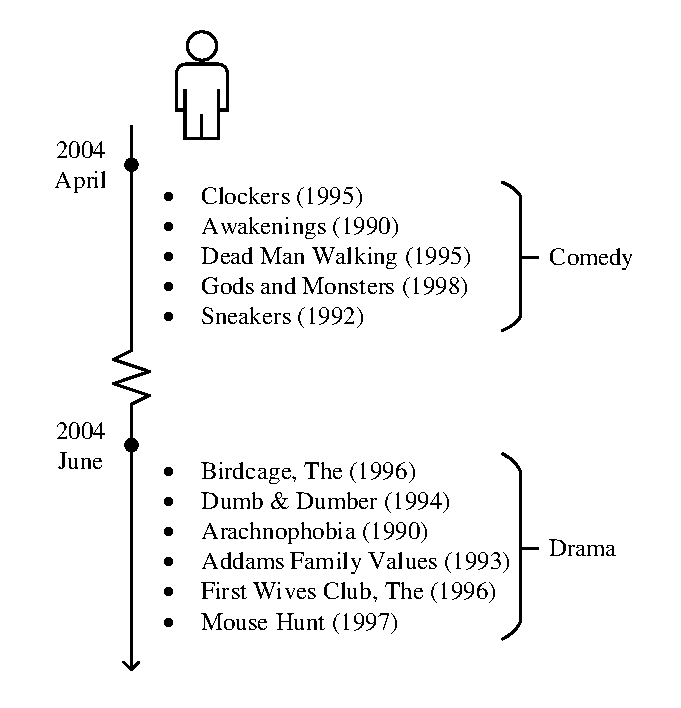
\includegraphics[scale=0.75]{images/example.pdf}
\caption{数据集MovieLens-1M中ID号为$5988$的用户的观影时间线}
\label{fig:example}
\end{figure}

例如,对于著名推荐系统数据集MovieLens-1M中一名ID号为$5988$的用户,
我们将他的电影评分数据按照时间进行排序,构成了图\ref{fig:example}所展示的观影时间线。
从图中我们可以观察得到,该用户在2004年四月份的时候热衷于观看喜剧类电影,
然后在2004年六月份开始转为喜爱观看戏剧类电影。

为了描述这种现象,本文提出了两个定义:长时间兴趣分布和短时间兴趣分布,
它们的具体描述如下:

\begin{enumerate}
\item \textbf{长时间兴趣分布}反映了用户在整个时间区间上的兴趣分布,
它体现在用户在整个时间区间上所有喜爱和讨厌的物品的整体集成上。
\item \textbf{短时间兴趣分布}反映了用户在某一固定时间子区间上的兴趣分布,
它体现在用户在这个固定时间子区间上所有喜爱和讨厌的物体的整体集成上。
\end{enumerate}

从两者的定义可以看出,一个用户可以拥有一个长时间兴趣分布和若干短时间兴趣分布。
在图\ref{fig:example}的例子中,ID号为$5988$的用户的长时间兴趣分布就是
既喜爱观看喜剧类电影又喜爱观看戏剧类电影,同时该用户又拥有两个短时间兴趣,
一个是四月份的喜爱观看喜剧类电影,另外一个是六月份喜爱观看戏剧类电影。

在传统协同过滤算法中,模型只考虑用户的长时间兴趣分布,
即这两个不同种类的电影由于同时被当前用户所喜爱而被同等对待处理,
但实际上它们的类型是不同的。
本文研究的起点就是研究如何更加合理地利用短时间兴趣分布来提高推荐系统的推荐性能。

下面我们将说明我们提出的两个新的假设,紧接着,我们介绍基于新假设的长短期兴趣模型,
最后我们利用长短期兴趣模型获得的用户特征和物品特征生成最终的评分结果。

\section{两个新的假设}
用户的长时间兴趣分布体现在整个时间区间中交互过的物品上,
短时间兴趣分布体现在若干时间子区间中交互过的物品上,
并且随着时间的推移不断发生变化,为了体现短时间兴趣分布的特点,
本文提出了两个新的假设,如下所示:

\begin{enumerate}
\item 对于同一个长时间兴趣分布中的若干短时间兴趣分布,
处于相同短时间兴趣分布中的物品之间的相似度大于
处于不同短时间兴趣分布中的物品之间的相似度。
\item 对于不同的长时间兴趣分布中的若干短时间兴趣分布,
物品同时出现在同一个短时间兴趣分布的次数和他们之间的相似度呈正相关关系,
即出现次数越多,物品之间的相似度越高,反之,出现次数越少,
物品之间的相似度越低。
\end{enumerate}

\begin{figure}[htbp]
\centering
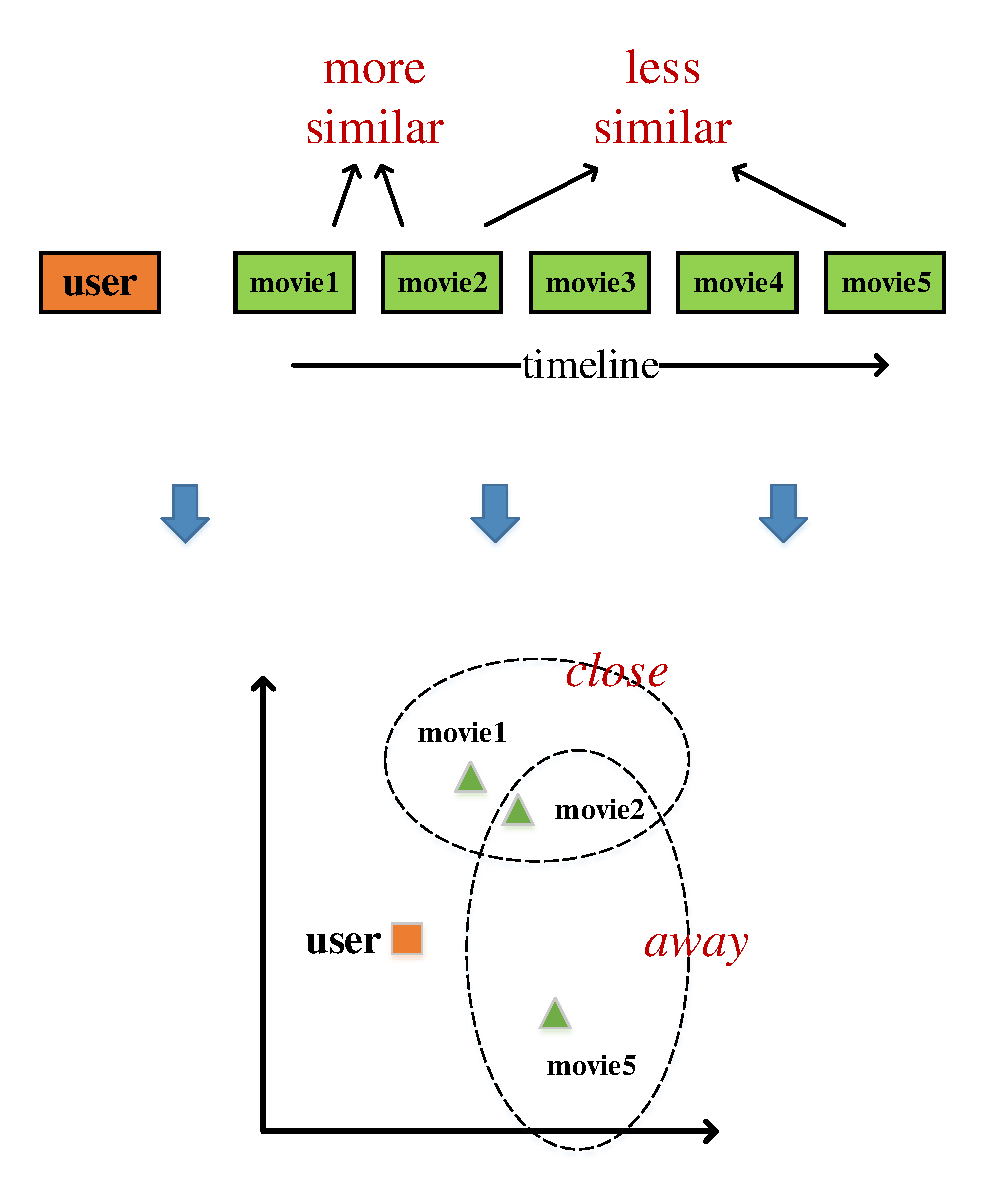
\includegraphics[scale=0.5]{images/embedding.pdf}
\caption{物品之间的相似度在低秩嵌入空间中的表现}
\label{fig:embedding}
\end{figure}

以图\ref{fig:embedding}为例,在图的上半部分,
用户$user$观看了$item1$,$item2$,$item3$,$item4$和$item5$五部电影,
我们将其按照时间进行排序,形成用户的观影时间线。
如果假设短时间的时间窗口长度为$2$,那么该用户就拥有$4$个短时间兴趣模型,
<$item1$,$item2$>,<$item2$,$item3$>,<$item3$,$item4$>和
<$item4$,$item5$>。
$item2$和$item1$处于同一个短时间兴趣分布,
$item2$和$item5$处于不同的短时间兴趣分布,
根据我们的第一个假设,
那么$item2$和$item1$的相似度应该大于$item2$和$item5$的相似度。
在图的下半部分,我们给出了在低秩嵌入空间中三者的空间位置,
通过向量之间的距离关系对应不同电影之间的相似度,
可以看到$item2$和$item1$的嵌入向量之间的距离小于
$item2$和$item5$的嵌入向量之间的距离。

\section{长短期兴趣模型}
自然语言处理Paragraph2Vec算法\parencite{le2014distributed}利用语句模型中
的单词顺序学习出有效的嵌入向量表示,在情感分类和信息检索任务上取得了较优的实验效果。
受到该算法的启发,本文提出了一个长短期兴趣模型(Long-Short Interest Model, LSIM),
基于提出的两个新的假设,从观影时间线中提取序列信息,
学习出更好的用户嵌入向量表示和物品嵌入向量表示。

\begin{figure}[htbp]
\centering
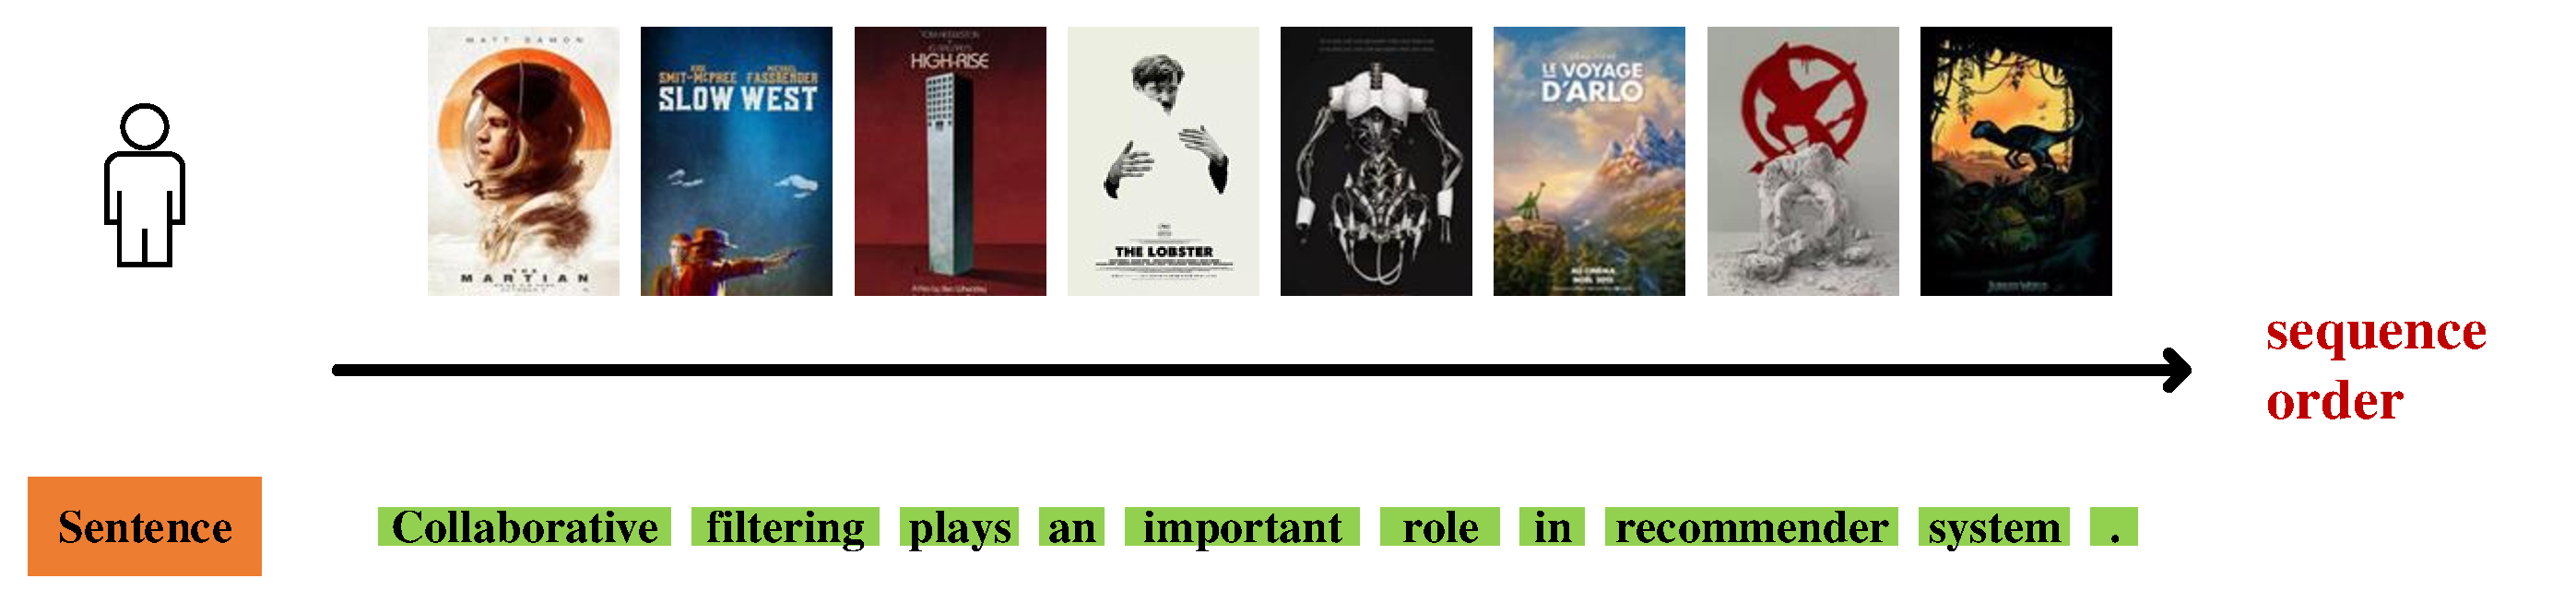
\includegraphics[scale=0.3]{images/example2.pdf}
\caption{Paragraph2vec learns vector representations of sentences and words
    based on the word order
    while LSIM extracts sequential features of users and items
    based on the rating order.
}
\label{fig:example2}
\end{figure}

如图\ref{fig:example2}所示,推荐算法中的用户类似于自然语言处理中的语句,
它们的共同点是都包含一个符合特定顺序关系的序列,
推荐短发中的物品类似于自然语言处理中的语句中的词语,
它们的共同点是都符合相对距离越近,相似程序越高的特点。

\begin{figure}[htbp]
    \centering
    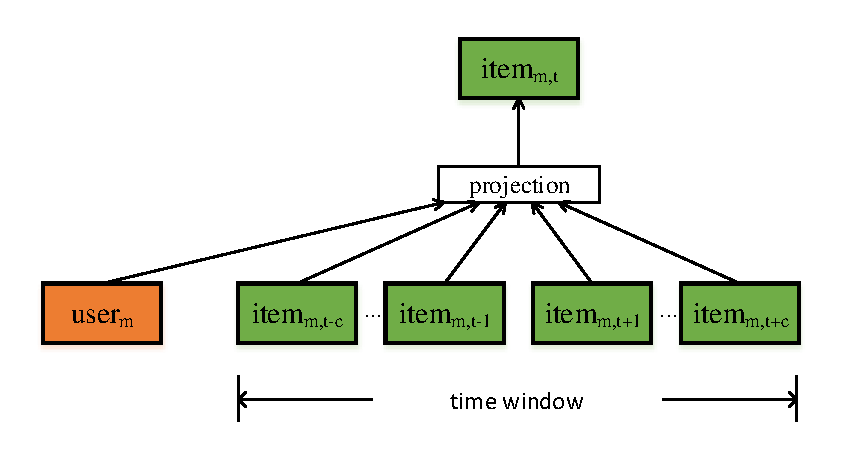
\includegraphics[scale=0.6]{images/doc2vec.pdf}
    \caption{Embedding Model for Extracting Interest Similarity from Users and Items}
    \label{fig:doc2vec}
\end{figure}

通过将用户作为一个全局的上下文信息,长短期兴趣同时学习出用户嵌入向量和物品嵌入向量,
整个模型的结构如图\ref{fig:doc2vec}所示。

假设推荐系统中存在$N$个用户$x_i(i \in 1,2,...,N)$以及$M$部电影$y_j(j \in 1,2,...,M)$
\footnote{我们使用符号$x和$y$代替经典的$u和$v$以避免符号$v$和向量符号$\mathbf{v}$在阅读上的误解},
每一个用户都拥有一个观影时间线$T_i(i \in 1,2,...,N)$,
包含了按照时间排序的若干电影信息$y_{i_1}$, $y_{i_2}$, ..., $y_{i_{L_i}}$,
其中$L_i$代表用户$x_i$观影时间线上电影的数量,其数值远远小于电影数量$M$。

为了建模长时间兴趣分布,我们考虑将整个观影时间线的电影作为上下文生成当前用户,
即
\begin{equation}
p(x_i | y_{i_1}, y_{i_2}, ..., y_{i_{L_i}})
\end{equation}

为了建模短时间兴趣分布,对于用户观影时间线上面的每一部电影,
我们考虑将用户和当前短时间窗口中的其他电影作为上下文来生成目标电影,
即
\begin{equation}
\sum_{j=1}^{L_i} p(y_{i_j} | y_{i_{j-c}} : y_{i_{j+c}}, x_i)
\end{equation}
其中$c$是时间窗口大小,$y_{i_{j-c}} : y_{i_{j+c}}$代表不包含
$y_{i_j}$项的序列$y_{i_{j-c}}, y_{i_{j-c+1}}, ..., y_{i_{j+c}}$。

所以更加正式地说,长短期兴趣模型的目标是最大化所有用户的
观影时间线$T_i(i \in 1,2,...,N)$的极大似然概率,
即
\begin{equation}
\sum_{i=1}^{N} \bigg( p(x_i | y_{i_1}, y_{i_2}, ..., y_{i_{L_i}}) +
\sum_{j=1}^{L_i} p(y_{i_j} | y_{i_{j-c}} : y_{i_{j+c}}, x_i) \bigg)
\end{equation}

其中$p(x_i | y_{i_1}, y_{i_2}, ..., y_{i_{L_i}})$是基于观看过的电影
生成$u_i$的长期兴趣的概率,这是一种典型的预测问题,我们可以使用多分类的方法解决,
例如Softmax,因此我们得到

\begin{equation}
p(x_i | y_{i_1}, y_{i_2}, ..., y_{i_{L_i}}) =
\frac
{
    exp ( \overline{\mathbf{v}}_{1}^{\mathrm{T}} \mathbf{v}_{x_i}^{'} )
}
{
    \sum_{x^{'}} exp ( \overline{\mathbf{v}}_{1}^{\mathrm{T}} \mathbf{v}_{x^{'}}^{'} )
}
\end{equation}

其中$\mathbf{v}_{x_i}^{'}$是用户$x_i$的输出向量表示,
$\overline{\mathbf{v}}_{1}$代表用户$x_i$的观影时间线上的所有电影的输入向量的平均值,
即
\begin{equation}
\overline{\mathbf{v}}_{1} = \frac{\sum_{j=1}^{T_i} \mathbf{v}_{y_{i_j}}}{T_i}
\end{equation}

而$p(y_{i_j} | y_{i_{j-c}} : y_{i_{j+c}}, x_i)$是使用用户长期兴趣和
同一个时间窗口内的其他电影生成$y_{i_j}$的概率,这也是一个多分类任务,
同样地,我们使用Softmax进行求解,即
\begin{equation}
p(y_{i_j} | y_{i_{j-c}} : y_{i_{j+c}}, x_i) =
\frac
{
    exp( \overline{\mathbf{v}}_{2}^{\mathrm{T}} \mathbf{v}_{y_{i_j}}^{'} )
}
{
    \sum_{y^{'}} exp( \overline{\mathbf{v}}_{2}^{\mathrm{T}} \mathbf{v}_{y^{'}}^{'} )
}
\end{equation}

其中$\mathbf{v}_{y_{i_j}}^{'}$代表电影$y_{i_j}$的输出向量表示,
$x_i$表示用户的长期兴趣向量表示
而$\overline{\mathbf{v}}_{2}$是同一个短期兴趣窗口内其他电影的向量表示的平均值,
即
\begin{equation}
\overline{\mathbf{v}}_{2} = \frac{
    \mathbf{v}_{x_i} + 
    \sum_{-c \leq k \leq c, k \not= 0}{\mathbf{v}_{y_{i_{j+k}}}}
}{2c+1}
\end{equation}

我们使用随机梯度下降(Stochastic Gradient Descent, SGD)对优化目标进行迭代求解,
同时层次Softmax(Hierarchical Softmax)和负采样(Negative Sampling)是
两个常见的计算加速算法,在本文中,我们使用负采样的方法进行计算加速。

\section{电影评分生成}
基于特征的协同过滤 \parencite{chen2011feature} 是协同过滤的一个变种,
和传统的矩阵分解不同的是,它允许我们在创建分解模型的同时利用诸多辅助信息,
例如用户画像,物品属性,好友关系和时间动态等等。

协同过滤中的特征一般可以分成两类:用户特征和物品特征,
我们使用$\mathbf{u}_i \in \mathbb{R}^{n}$代表用户特征,
$\mathbf{v}_j \in \mathbb{R}^{m}$代表物品特征,
那么预测评分数值$\hat{r}$ 的公式为

\begin{equation}
\hat{r}_{ij} = \sum_{k=1}^{n} \alpha_k \mathbf{u}_{ik} + \sum_{k=1}^{m} \beta_k \mathbf{v}_{jk} +
\left( \sum_{k=1}^{n} \mathbf{u}_{ik} \mathbf{p}_k \right) ^ \mathrm{T}
\left( \sum_{k=1}^{m} \mathbf{v}_{jk} \mathbf{q}_k \right)
\end{equation}

其中$\alpha$和$\beta$分别控制着用户特征和物品特征的影响程度
$\mathbf{p}_{k} \in \mathbb{R}^K$和$\mathbf{q}_{k} \in \mathbb{R}^K$
是$K$维的和每一个特征相关的隐向量因子。
如果我们使用独热向量(One-Hot Representation)来表示用户和物品,即
\begin{equation}
\mathbf{u}_{ik} =
\left\{
\begin{aligned}
1, &k = i \\
0, &k \not= i
\end{aligned}
\right. \\ , 
\mathbf{v}_{jk} =
\left\{
\begin{aligned}
1, &k = j \\
0, &k \not= j
\end{aligned}
\right. \\
\end{equation}

那么上文中的评分预测公式就会退化为基本的矩阵分解算法,
即
\begin{equation}
\hat{r}_{ij} = \alpha_i + \beta_j + \mathbf{p}_i ^ \mathrm{T} \mathbf{q}_j
\end{equation}

其中$\alpha$和$\beta$分别代表用户偏移和物品偏移,
而$\mathbf{p}_i$和$\mathbf{q}_j$分别代表用户$\mathbf{u}_i$和物品$\mathbf{v}_j$
对应的隐向量因子。


在本文的工作中,我们使用长短期兴趣模型中学习出来的用户表示和物品作为一种辅助信息。
因此,我们定义$\tilde{\mathbf{u}}_i$代表学习出来的用户表示,
$\tilde{\mathbf{v}}_j$代表学习出来的物品表示。
然后,我们通过组合学习出的用户物品表示和经典的独热表示得到新的特征组合,即

\begin{equation}
\mathbf{u}_{i} = \{ \mathbf{u}_{i} , \tilde{\mathbf{u}}_i \} , 
\mathbf{v}_{j} = \{ \mathbf{v}_{j} , \tilde{\mathbf{v}}_j \}
\end{equation}

因此评分预测的公式将会变为

\begin{equation}
\begin{aligned}
\hat{r}_{ij} =
&\sum_{k=1}^{N+D} \alpha_k \{ \mathbf{u}_i , \tilde{\mathbf{u}}_i \}_k +
\sum_{k=1}^{M+D} \beta_k  \{ \mathbf{v}_j , \tilde{\mathbf{v}}_j \}_k + 
&\left( \sum_{k=1}^{N+D} \{ \mathbf{u}_i , \tilde{\mathbf{u}}_i \}_k \mathbf{p}_k \right) ^ \mathrm{T}
\left( \sum_{k=1}^{M+D} \{ \mathbf{v}_j , \tilde{\mathbf{v}}_j \}_k \mathbf{q}_k \right)
\end{aligned}
\end{equation}

其中$N$是推荐系统中的用户的数量,$M$是推荐系统中物品的数量,
$D$本文提出的长短期兴趣模型中学习出来的用户特征和物品特征的维度,
$\mathbf{p}_{k} \in \mathbb{R}^K$和$\mathbf{q}_{k} \in \mathbb{R}^K$
是$K$关联到每个特征的隐向量因子的维度。



	\chapter{实验及结果分析}

	\chapter{电影推荐系统的设计与实现}


	% 正文中的附录部分。
	\appendix
	% 排版参考文献列表。bibintoc 选项使“参考文献”出现在目录中;
	% 如果同时要使参考文献列表参与章节编号,可将“bibintoc”改为“bibnumbered”。
	\printbibliography[heading = bibintoc]
	% 各附录。
	% Copyright (c) 2014,2016 Casper Ti. Vector
% Public domain.

\chapter{攻读硕士学位期间的科研成果}
\begin{itemize}
\item \textbf{Chao Lv}, Lili Yao, Yansong Feng and Dongyan Zhao. Improving Collaborative Filtering with Long-Short Interest Model. NLPCC 2016.
\item \textbf{Chao Lv}, Yansong Feng and Dongyan Zhao. Purchase Prediction via Machine Learning in Mobile Commerce. NLPCC 2016.
\item \textbf{Chao Lv}, Runwei Qiang, Feifan Fan and Jianwu Yang. Knowledge-based Query Expansion in Real-Time Microblog Search. AIRS 2015.
\item \textbf{Chao Lv}, Runwei Qiang, Lili Yao and Jianwu Yang. EEST: Entity-driven Exploratory Search for Twitter. AIRS 2015.
\item \textbf{Chao Lv}, Feifan Fan, Runwei Qiang, Yue Fei and Jianwu Yang. PKUICST at TREC 2014 Microblog Track: Feature Extraction for Effective Microblog Search and Adaptive Clustering Algorithms for TTG. TREC 2014.
\item Yue Fei, \textbf{Chao Lv}, Yansong Feng and Dongyan Zhao. Real-time Filtering on Interest Profiles in Twitter Stream. JCDL 2016.
\item Lili Yao, \textbf{Chao Lv}, Feifan Fan, Jianwu Yang, Dongyan Zhao PKUICST at TREC 2016 Real-Time Summarization Track: Push Notifications and Email Digest. TREC 2016.
\item Feifan Fan, Yue Fei, \textbf{Chao Lv}, Lili Yao, Jianwu Yang and Dongyan Zhao. PKUICST at TREC 2015 Microblog Track: Query-biased Adaptive Filtering in Real-time Microblog Stream. TREC 2015.
\item Feifan Fan, Runwei Qiang, \textbf{Chao Lv} and Jianwu Yang. Improving Microblog Retrieval with Feedback Entity Model. CIKM 2015.
\item Feifan Fan, Runwei Qiang, \textbf{Chao Lv}, Wayne Xin Zhao and Jianwu Yang. Tweet Timeline Generation via Graph-based Dynamic Greedy Clustering. AIRS 2015.
\item \textbf{吕超},强闰伟,姚丽丽,杨建武,``一种基于多来源实体驱动的探索性微博检索系统'',专利号:201510246802.5
\end{itemize}


	% 以下为正文之后的部分,默认不进行章节编号。
	\backmatter
	% 致谢。
	\chapter{致谢}
从论文的选题、资料的收集、实验的安排和论文的撰写整个过程中,我得到了许多热情的帮助。

首先,我要由衷感谢北京大学给我提供了良好的学习氛围,
2014级信息科学技术学院这个集体带领了我进入了计算机科学研究的世界,
同周围的同学们一起学习,一起进步的三年将成为我一生中最美好的记忆。

感谢我的导师赵东岩老师和冯岩松老师,两位老师无论在学习上还是工作上都给予了我充分的指导和关怀,
并以自己丰富的阅历在学术和为人处世方面给了我诸多教导,使我获益良多。
你们严谨的工作态度、渊博的学识、平易近人的待人方式和诲人不倦的师长风范都为了树立了良好的学习榜样。

感谢我的另一位导师杨建武老师,是您的悉心指导引领我进入了学术的殿堂,为我的研究生涯铺平了道路,
并且给予了我无形的精神鼓励。感谢我的班主任张行功老师以及研究所的戴永宁老师、姚春霞老师、 鞠莉老师、韩玉晶老师和张猛老师,感谢她们在生活上和学习上对我的关心和鼓励。

感谢强闰伟师兄对我生活和学习上的悉心帮助,他在平日的研究工作中努力认真,
积极进取,在生活中乐观开朗,给我即将到来的研究生生活树立了一个优秀的榜样。
同时也感谢研究所洪毅虹师姐、费跃师兄和姚丽丽师妹的帮助和鼓励,
感谢他们在新的环境中鼓励我迎难而上,在追求科研和学术的道路上永不停步。

最后要感谢的是我的家人,他们无私的关怀是我努力进取的动力,使我永远不会感觉孤单和疲倦。
在未来的日子里,我会更加努力的学习和工作,不辜负家人对我的殷殷期望。
特别感谢王慧,感谢你出现在我的生命里,在我失落时给予我关怀与鼓励,
在我骄傲时给我当头一棒,让我继续努力。

最后,对参加论文评审、答辩的各位老师表示衷心的感谢!



	% 原创性声明和使用授权说明。
	% Copyright (c) 2008-2009 solvethis
% Copyright (c) 2010-2017 Casper Ti. Vector
% All rights reserved.
%
% Redistribution and use in source and binary forms, with or without
% modification, are permitted provided that the following conditions are
% met:
%
% * Redistributions of source code must retain the above copyright notice,
%   this list of conditions and the following disclaimer.
% * Redistributions in binary form must reproduce the above copyright
%   notice, this list of conditions and the following disclaimer in the
%   documentation and/or other materials provided with the distribution.
% * Neither the name of Peking University nor the names of its contributors
%   may be used to endorse or promote products derived from this software
%   without specific prior written permission.
%
% THIS SOFTWARE IS PROVIDED BY THE COPYRIGHT HOLDERS AND CONTRIBUTORS "AS
% IS" AND ANY EXPRESS OR IMPLIED WARRANTIES, INCLUDING, BUT NOT LIMITED TO,
% THE IMPLIED WARRANTIES OF MERCHANTABILITY AND FITNESS FOR A PARTICULAR
% PURPOSE ARE DISCLAIMED. IN NO EVENT SHALL THE COPYRIGHT HOLDER OR
% CONTRIBUTORS BE LIABLE FOR ANY DIRECT, INDIRECT, INCIDENTAL, SPECIAL,
% EXEMPLARY, OR CONSEQUENTIAL DAMAGES (INCLUDING, BUT NOT LIMITED TO,
% PROCUREMENT OF SUBSTITUTE GOODS OR SERVICES; LOSS OF USE, DATA, OR
% PROFITS; OR BUSINESS INTERRUPTION) HOWEVER CAUSED AND ON ANY THEORY OF
% LIABILITY, WHETHER IN CONTRACT, STRICT LIABILITY, OR TORT (INCLUDING
% NEGLIGENCE OR OTHERWISE) ARISING IN ANY WAY OUT OF THE USE OF THIS
% SOFTWARE, EVEN IF ADVISED OF THE POSSIBILITY OF SUCH DAMAGE.

{
	\ctexset{section = {
		format+ = {\centering}, beforeskip = {40bp}, afterskip = {15bp}
	}}

	% 学校书面要求本页面不要页码,但在给出的 Word 模版中又有页码且编入了目录。
	% 此处以 Word 模版为实际标准进行设定。
	\specialchap{北京大学学位论文原创性声明和使用授权说明}
	\mbox{}\vspace*{-3em}
	\section*{原创性声明}

	本人郑重声明:
	所呈交的学位论文,是本人在导师的指导下,独立进行研究工作所取得的成果。
	除文中已经注明引用的内容外,
	本论文不含任何其他个人或集体已经发表或撰写过的作品或成果。
	对本文的研究做出重要贡献的个人和集体,均已在文中以明确方式标明。
	本声明的法律结果由本人承担。
	\vskip 1em
	\rightline{%
		论文作者签名:\hspace{5em}%
		日期:\hspace{2em}年\hspace{2em}月\hspace{2em}日%
	}

	\section*{%
		学位论文使用授权说明\\[-0.33em]
		\textmd{\zihao{5}(必须装订在提交学校图书馆的印刷本)}%
	}

	本人完全了解北京大学关于收集、保存、使用学位论文的规定,即:
	\begin{itemize}
		\item 按照学校要求提交学位论文的印刷本和电子版本;
		\item 学校有权保存学位论文的印刷本和电子版,
			并提供目录检索与阅览服务,在校园网上提供服务;
		\item 学校可以采用影印、缩印、数字化或其它复制手段保存论文;
		\item 因某种特殊原因需要延迟发布学位论文电子版,
			授权学校在 $\Box$\nobreakspace{}一年 /
			$\Box$\nobreakspace{}两年 /
			$\Box$\nobreakspace{}三年以后在校园网上全文发布。
	\end{itemize}
	\centerline{(保密论文在解密后遵守此规定)}
	\vskip 1em
	\rightline{%
		论文作者签名:\hspace{5em}导师签名:\hspace{5em}%
		日期:\hspace{2em}年\hspace{2em}月\hspace{2em}日%
	}

	% 若需排版二维码,请将二维码图片重命名为“barcode”,
	% 转为合适的图片格式,并放在当前目录下,然后去掉下面 2 行的注释。
	\vfill\noindent
	
\includegraphics[height = 5em]{barcode}
}

% vim:ts=4:sw=4

\end{document}

% vim:ts=4:sw=4
